\documentclass{article}
\usepackage{a4wide}
\usepackage{graphicx}
\usepackage{amsmath, amsthm, amssymb}
\usepackage{mathrsfs}
% GOTH FONT 
% \usepackage{yfonts}
% \AtBeginDocument{\gothfamily}
\usepackage[utf8]{inputenc}
\usepackage{ngerman}
\usepackage{url}
\usepackage[ruled,vlined]{algorithm2e}
\usepackage[]{hyperref}
\usepackage{listings}
\usepackage{dsfont}

\newtheorem{thm}{Theorem}[section]
\newtheorem{cor}[thm]{Korollar}
\newtheorem{lem}[thm]{Lemma}
\newtheorem{defi}[thm]{Definition}
\newtheorem{definition}{Definition}
\newcounter{Chapcounter}
\newcommand\showmycounter{\addtocounter{Chapcounter}{1}\themycounter}
\newcommand{\chapter}[1] 
{ {\centering          
  \addtocounter{Chapcounter}{1} \Large \underline{\textbf{ \color{blue} Chapter \theChapcounter: ~#1}} }   
  \addcontentsline{toc}{section}{ \color{blue} Chapter:~\theChapcounter~~ #1}    
}
\hypersetup{colorlinks=true}
\hypersetup{linkcolor=black}
\usepackage{listings}
\lstdefinelanguage{Pseudo}{
  morekeywords={forall,if,then,else,return,while,do,for,DFS},
  sensitive=false,
  morecomment=[l]{//},
  morestring=[b]"
}



\setcounter{tocdepth}{4}

\begin{document}
\title{Foundations of Machine Learning}
\date{Sommersemester 2026}
\author{Universität Stuttgart}
\maketitle
\tableofcontents
\newpage
\section{Preface}
These notes are mainly written in English, but there may be a few words in German and/or Spanish, since English is not my native language.

These notes contain all topics I valued as important for the exam, but some stuff that may have been trivial for me may not appear in the notes. So if anybody is using my notes to 
prepare for the exam, please be wary of this.

\section{Ultra-Mega-basics}
\[(AB)^T = B^TA^T\]
Positive definite matrix:
\[x^T Ax > 0 \forall x \neq 0\]
Regular matrix
\[A^{-1} \text{ exists}\]

Vector derivatives
Let $x \in \mathbb{R}^n$. What is $\frac{\partial}{\partial x}x$?

Solution: $\frac{\partial}{\partial x}x = (\frac{\partial x_i}{\partial x_j})_{i = 1,\dots,n; j=1,\dots,n}$. So its an $n\times n$ matrix of all combinations of the derivatives.

Derivative of a scalar in respect to a vector is now a row vector.
\[\frac{\partial}{\partial x}x^T \cdot x = [\frac{\partial}{\partial x_i}x_1^2 + \dots + x_n^2]_{1\leq i \leq n} = [2x_i]_{1\leq i \leq n}\]

\textbf{NOTE: This a standard, not the universal truth}

We define $r_i := y_i - \hat{y}_i$

Mean Squared Error
\[MSE(y,\hat{y}) = \frac{1}{n}\sum_{i=1}^{n}r_i^2\]
Mean Absolute Error
\[MAE(y,\hat{y}) = \frac{1}{n}\sum_{i=1}^{n}|r_i|\]

Recommended Linear Algebra videos MIT by some guy dont remember the name

$\propto$ Means proportional to.

$D = \{x_1,\dots,x_n\} \subseteq X_1\times\dots\times X_m$ means that the dataset has $n$ objects/observations, each of them having m attributes. $X_m$ represents the set of values that attribute can take.  
\section{Organizational}
Exam is in theory on August 13.

It is recommended to have attended before 'Foundations of Artificial Intelligence'

Coding in Python

\subsection{How to get the Schein}
\begin{itemize}
  \item 11 Assignments, submission of three members
  \item Exam admission on an individual basis
  \item Present solutions twice (once in first 5 excersises, once in remaining sessions)
  \item Just have to give in excersises, don't seem that they are corrected.
\end{itemize}
\section{Introduction}

\subsection{What is Machine Learning?}
A computer is said to learn:
\begin{itemize}
  \item from experience $E$
  \item with respect to a task $T$
  \item and a performance measure $P$
\end{itemize}
if its performance on $T$, measured by $P$, improves with experience $E$.

\subsection{What Does ML Learn?}

\subsubsection{Regression}
Given a set of existing values, predict a continuous output.

\textbf{Example:} Predicting daily temperature.

Experience $E$ is typically a set of tuples $(x, y)$, where:
\begin{itemize}
  \item $x$: input (e.g., date)
  \item $y$: output (e.g., temperature)
\end{itemize}

Goal: find a function
\[
\hat{f}(x) \approx y
\]

This prediction process is called \textbf{inference}.

\textbf{Output:} continuous values

\subsubsection{Classification}
Assign input values to discrete classes.

\textbf{Example:} Determining whether a dog in an image is dangerous or not.

Experience consists of pairs (input, class label).

The prediction is also called \textbf{inference}.

\textbf{Output:} discrete values

\subsubsection{Supervised Learning}
Assume there exists a ground truth function:
\[
f : X \to Y
\]

Given training data $D$, the goal is to find $\hat{f}$ such that it approximates $f$ as closely as possible (measured using $P$).

\subsubsection{Reinforcement Learning}
Starts with no prior experience, but with a policy (strategy).

\begin{enumerate}
  \item Choose an action based on the current policy
  \item Observe the outcome and receive a reward
  \item Update the policy based on the reward
  \item Repeat
\end{enumerate}

\subsubsection{Unsupervised Learning}
No target values and no explicit rewards -- only raw data.

\paragraph{Data Clustering}
Data points are grouped into clusters based on similarity.

Idea:
\begin{itemize}
  \item Points in the same cluster are more similar to each other
  \item Points in different clusters are less similar
\end{itemize}

Used to uncover hidden patterns in data.

\section{Terminological Chaos}
\textbf{Warning:} There is quite a bit of inconsistent terminology in this field.

(See lecture slides for a more detailed breakdown.)

\begin{itemize}
  \item Pattern recognition $\approx$ supervised learning
  \item Data mining $\neq$ strict synonym for knowledge discovery
\end{itemize}

\section{Knowledge Discovery}
The non-trivial process of identifying valid, novel, and useful patterns in data.

\subsection{Problem of Knowledge Discovery}
Given input data $D$, find a pattern $S$ such that:
\begin{itemize}
  \item $S$ is an expression in an understandable language $L$ describing correlations in $D$, and likely describve a new data $D^{new}$
  \item $S$ is simpler than $D$
\end{itemize}

\subsection{Stages of Knowledge Discovery}
\begin{enumerate}
  \item Data selection (choose relevant data)
  \item Data cleaning
  \item Data transformation (convert into usable format)
  \item Data mining (search for patterns)
  \item Evaluation (assess discovered patterns)
  \item Knowledge representation (present results to users)
\end{enumerate}

\section{The Crisp-DM model}

\begin{center}
  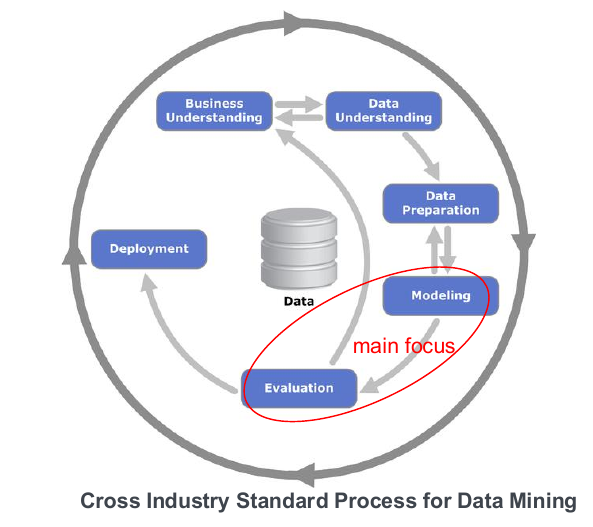
\includegraphics[scale=0.7]{assets/crisp-dm-model.png}
\end{center}

\subsection{Business Understanding}
\begin{enumerate}
  \item Determine Business objectives: define success criteria.
  \item Assess Situation (Risks, Resorces, Costs, Benefits...)
  \item Determine Data Mining Goals
  \item Produce Project Plan
\end{enumerate}

\subsection{Data Understanding}
\begin{itemize}
  \item Collect initial data: Identify relevant attributes, inconsistencies.
  \item Describe data: Statistical models for the data (mean, median...). Correlation between attributes.
  \item Explore Data
  \item Verify Data Quality: Errors in the data, missing values, false encodings...
\end{itemize}

\paragraph{Statistical Descriptions}
\begin{itemize}
  \item \textbf{Mode: }most frequent value. Always applicable

  \item \textbf{Median: }$\tilde{x}$ middle value. Only applicable to ordinal, interval and ratio scales.

  \item \textbf{Mean: } $\mu = \mathbb{E}_{x\in X}[x] = \frac{1}{n}\sum_{i=1}^{n}x_i$. Applicable to interval and ratio scales.

  \item \textbf{Standard deviation: } $\sigma^2 = \mathbb{E}_{x\in X}[(x-\mu)^2] =\frac{1}{n-1}\sum_{i=1}^{n}(x_i-\mu)^2$

  \item \textbf{Fisher-Pearson skewness: }$\mathbb{E}_{x\in X}[(\frac{x-\mu}{\sigma})^3]$
  
\end{itemize}

\paragraph{Quartiles and Quantiles} 1st, 2nd, 3rd, 4th Quartile

\[IQR = Q_3 - Q_1\]

Outliers are values beyond \textbf{Tukey's fence}
\[[Q_1-k\cdot IQR, Q_3 + k\cdot IQR]\]
for $k=1.5$ or $k=3$

\subsection{Data Preparation}
\begin{itemize}
  \item Select data (feature selection): only get useful attributes. Discard highly correlated attributes
  \item Integrate data: Mix data from different sources. Careful with syntax/semantics/units of measurements.
  \item Clean Data: Correct false values, remove outliers, estimate missing values
  \item Format Data
  \item Feature Engineering: Define features from attribtes (e.g convert coordinates to distance). Normalize/transform single attributes.
\end{itemize}
\subsubsection{Categorical data to numeric: 1-hot encoding}
Given dataset $D = \{x_1,\dots,x_n\} \subseteq X_1\times\dots\times X_m$

Categorical attribute $X_j$ with categories $dom(X_j) = \{a_1,\dots,a_k\}$

Define $\hat{X_j}\subseteq\{0,1\}^k$ and
\[\hat{x_{i,j,l}} = \begin{cases}
  1 \quad j = l\\
  0 \quad else
\end{cases}\]
Imagine it as a 3-D table with ones and zeroes.

Struggles with scalability and sparcity issues.

\subsubsection{Categorical data to numeric: Target encoding}
Categorical attribute $A$ with categories $dom(A) = \{a_1,a_2,\dots,a_k\}$

Given target attribute Y with $dom(Y) = \{0,1\}$

Given dataset $D\subseteq A\times X \times Y$

\[\hat{a_i} = \frac{|\{a_i,.,1\}\in D|}{|\{a_i,.,.\}\in D|} \in [0,1]\]
\[\hat{a}^{(i)} = \frac{\text{Nº times category } a^{(i)} \text{ appears with } Y=1} {\text{Nº times category } a^{(i)} \text{ appears}}\]

Replace occurrances of $a_i$ with $\hat{a_i}$

Struggles with overfitting and bias
\subsubsection{Numerical data to nominal data}
Given dataset $D = \{(x_1,y_1),\dots,(x_n,y_n)\}\subseteq X\times Y $

Given $X = \mathbb{R}$

Define $\hat{X} = \{1,\dots,k\}, k\geq 2$

Problem: Define $\hat{D}$ to represent original learning problem well. So we want to be able to group the values into $k$ \textbf{bins}.

For $k=2$ take median to decide between bin 1 or 2

\subsection{Modeling}
\subsubsection{Select Modeling Technique}
Take into account experience, and requirements. Generate a \textbf{Test Design} with data sets for \textbf{training data}, \textbf{validation data} and \textbf{test data}

Build and assess model
\subsection{Evaluation}
Define evaluation criteria during business understanding.

\begin{itemize}
  \item Evaluate results: Findings of the project. \textbf{Algorithm must not determine business evaluation}
  \item Review process: Identify failures
  \item Determine next steps
\end{itemize}


\subsection{Deployment}
\begin{itemize}
  \item Plan deployment: target platform, mobile, sensor quality\dots
  \item Plan Monitoring and Maintenance
  \item Produce Final Report
  \item Review Project
\end{itemize}

\section{Dimensionality Reduction}
Thought experiment: See around in your room, then close your eyes, and try to predict what will happen. Your prediction will of course not be a 1:1 representation of the room to the pixel level. Your predictions are semantic, where that guy is moving, where that ball will land, etc.

So the conclusion from this, is that to some extent the information is compressed, removing noise and more.

The basis of machine learning is that human predictions and experiences are low dimensional. This is because we ourselves as humans can predict pretty well.

\paragraph{Mathematics}: The mathematics of predictions are probability distributions $P(X)$ of low-dimensional support (manifold) in high-dimensional data space. Translated: we just look at a relevant subspace for the prediction. 

\paragraph{Principle of parsimony}: Learn a low-dimensional representation (from $10^4-10^{10}$ dimensions to $10^0-10^3$ dimensions)

\subsection{How to reduce dimensionality}
The problem is the high dimensionality of data
\begin{itemize}
  \item Images: $\mathbb{R}^{3\times 200\times 300}$ (or more)
  \item Documents represented as bag-of-words. Each document counts occurances of each term. $tf(d,t)$. Represented by vector in $\mathbb{R}^{10000}$ or more.
\end{itemize}

The idea is to find the \textbf{most} important dimensions.

\subsubsection{(Semi)Formal definition of dimensionality reduction}
Given data set $\mathcal{D} = \{x_1,...,x_N\}\subseteq \mathbb{R}^D$

Find a function $\hat{f} : \mathbb{R}^D\to \mathbb{R}^d$ with $d<<D$
to derive a data set $\hat{\mathcal{D}} = \{\hat{f}(x_1),...,\hat{f}(x_N)\} \subseteq \mathbb{R}^d$

such that the main characteristics are preserved

If the main characteristics are formalized, it's an optimization problem

\[\mathcal{L}(\hat{f}) = \sum_{i=1}^{N}(x_i - \hat{f}^{-1}(\hat{f}(x_i)))^2\]
This counts basically the 'information loss'. And we want to minimize that.

\subsection{Dimensionality Reduction techniques}
\subsubsection{Linear Transformations Refresher}
Given $x = (x_1,x_2)^T\in\mathbb{R}^2$

We can
\begin{itemize}
  \item Scale by $s_1,s_2$ with 
  \[\begin{pmatrix}
    s_1 & 0 \\
    0 & s_2
  \end{pmatrix}\cdot x\]
  \item Rotate by $\varphi$
  \[\begin{pmatrix}
    \cos\varphi & -\sin\varphi \\
    \sin\varphi & \cos\varphi
  \end{pmatrix}\cdot x\]
  \item Project onto one axis
  \[\begin{pmatrix}
    1 & 0 \\
    0 & 0
  \end{pmatrix}\cdot x = (x_1,0)^T\]
\end{itemize}
\subsubsection{Sample Covariance Matrix Refresher}
Given data set $\mathcal{D} = \{x_1,...,x_N\}\subseteq \mathbb{R}^D$

There are N data points, each with D dimensions. So we can represent everything as a $N\times D$ matrix.
\[X = \begin{pmatrix}
  x_{1,1} & \dots & x_{1,D}\\
  \vdots & \ddots & \vdots \\
  x_{N,1} & \dots & x_{N,D}
\end{pmatrix}\]

And we can compute the \textbf{sample covariance matrix} $\hat{\Sigma} = [q_{j,k}] \in \mathbb{R}^{D\times D}$
\[q_{j,k} = \frac{1}{N-1}\sum_{i=1}^N(x_{i,j} - \overline{x}_j)(x_{i,k} - \overline{x}_{k})\]

Intuitively, it measures how different features (dimensions) move together
\begin{itemize}
  \item $(x_{i,j}-\overline{x}_j$) asks, for observation $i$, is feature $j$ above or below its average?
  \item $(x_{i,k}-\overline{x}_k$) asks, for observation $i$, is feature $k$ above or below its average?
\end{itemize}
Positive covariance means both features rise or decrease at the same time, like for example, as house size increases, it's price does also. Negative covariance is the inverse, car weight vs gas mileage. Zero (or close to it) means no relationship
\subsubsection{Principal Component Analysis (PCA)}
Assume that $\hat{f}$ is linear.
\[\hat{f}(x) = Vx\]

Then the loss is
\[\mathcal{L}(\hat{f}_V) = \mathcal{L}(V) = \frac{1}{N}\sum_{i=1}^{N}(x_i - \hat{f}_V(x_i))^2\]

\paragraph{Idea of PCA: }Given the usual dataset $\mathcal{D}$, first of all translate the data so that $\sum_{i=1}^{N}x_i = 0$

Represent it as the $N\times D$ matrix $X$

\begin{enumerate}
  \item Rotate and project the data onto the \textbf{most important dimension}
  \item Subtract this part
  \item Repeat from 1
\end{enumerate}
\begin{center}
  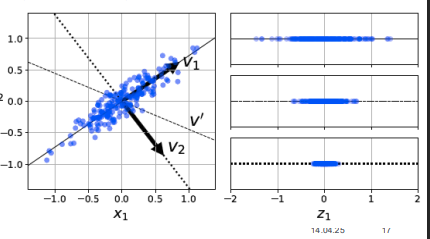
\includegraphics[scale=0.7]{assets/pca.png}  
\end{center}

In this case, the most important dimension is $V_1$
\paragraph{Finding the best $d$ axes (PCA)}

We are given data points:
\[
x_1, x_2, \dots, x_N \in \mathbb{R}^D
\]

Goal:
\begin{itemize}
    \item Find $d$ orthonormal vectors (axes)
    \[
    v_1, v_2, \dots, v_d \in \mathbb{R}^D, \quad \|v_j\| = 1, \; v_i^\top v_j = 0 \ (i \neq j)
    \]
    \item Find new coordinates for each data point:
    \[
    z_i = (z_{i,1}, \dots, z_{i,d}) \in \mathbb{R}^d
    \]
\end{itemize}

We approximate each point as:
\[
x_i \approx \sum_{j=1}^d z_{i,j} v_j
\]

The reconstruction error is:
\[
\mathcal{L}(V,Z) = \frac{1}{N} \sum_{i=1}^N \left\| x_i - \sum_{j=1}^d z_{i,j} v_j \right\|^2
\]

\textbf{Goal:} Minimize this error.

\vspace{0.5em}
\paragraph{Finding the first axis}

We first solve for one direction $v_1$:

\[
\mathcal{L}(v_1, z_{\cdot,1}) = \frac{1}{N} \sum_{i=1}^N \|x_i - z_{i,1} v_1\|^2
\]

Expanding:
\[
= \frac{1}{N} \sum_{i=1}^N \left( x_i^\top x_i - 2 z_{i,1} v_1^\top x_i + z_{i,1}^2 \right)
\]

Optimize for $z_{i,1}$ (equal partial derivative to zero and clear up (computation skipped, directly give result)):
\[
\frac{\partial}{\partial z_{i,1}}\mathcal{L}(v_1,z_{.,1}) = 0 \quad \Rightarrow \quad z_{i,1} = v_1^\top x_i
\]

\textit{(This is the projection of $x_i$ onto $v_1$)}

Plugging back:
\[
\mathcal{L}(v_1) = \frac{1}{N} \sum_{i=1}^N \left( x_i^\top x_i - (v_1^\top x_i)^2 \right)
\]

\[
= \underbrace{\text{const}}_{\text{Represents the } x_i^Tx_i \text{ stuff}} - \frac{1}{N} \sum_{i=1}^N v_1^\top x_i x_i^\top v_1
\]

Define empirical covariance:
\[
\hat{\Sigma} = \frac{1}{N} \sum_{i=1}^N x_i x_i^\top
\]

Then:
\[
\mathcal{L}(v_1) = \text{const} - v_1^\top \hat{\Sigma} v_1
\]

So minimizing $\mathcal{L}$ is equivalent to maximizing:
\[
v_1^\top \hat{\Sigma} v_1
\quad \text{subject to } \|v_1\| = 1
\]

\vspace{0.5em}
\paragraph{Optimization via Lagrange multipliers}

\[
\mathcal{L}'(v_1) = v_1^\top \hat{\Sigma} v_1 - \lambda (v_1^\top v_1 - 1)
\]

Set derivative to zero:
\[
\hat{\Sigma} v_1 = \lambda v_1
\]

\textbf{Result:}
\begin{itemize}
    \item $v_1$ is an eigenvector of $\hat{\Sigma}$
    \item Choose the eigenvector with the \textbf{largest eigenvalue} (Why? See below)
\end{itemize}
We want to maximize $v_1^T\hat{\Sigma}v_1$ and we already saw that $\hat{\Sigma}v_1 = \lambda v_1$ so we can replace

\[v_1^T\hat{\Sigma}v_1 = v_1^T\lambda v_1 = \lambda \underbrace{v_1^Tv_1}_{=1} = \lambda\]
So maximizing lambda maximizes the function from before.

\vspace{0.5em}
\paragraph{Induction step (more axes)}

For additional axes:
\begin{itemize}
    \item $v_2, v_3, \dots, v_d$ must be orthogonal to previous ones
    \item Each maximizes variance in remaining directions
\end{itemize}

\textbf{Result:}
\begin{itemize}
    \item $v_j$ = eigenvector of $\hat{\Sigma}$
    \item Corresponding to the $j$-th largest eigenvalue
\end{itemize}

\vspace{0.5em}
\paragraph{Final interpretation}

\begin{itemize}
    \item PCA finds directions of \textbf{maximum variance}
    \item Projects data onto a lower-dimensional space
    \item Minimizes reconstruction error
\end{itemize}

\vspace{0.5em}
\paragraph{Intuition}

\begin{itemize}
    \item $d = D$: no information loss, just rotation
    \item $d < D$: compress data while keeping most important structure
\end{itemize}
\section{Cluster Analysis}
\subsection{Goal of clustering}
Identifying 'clusters' or 'groups' in the data, where objects in the same group are as similar as possible. Objects in different clusters should be as dissimilar as possible.

In \textbf{unsupervised learning}, no specific groups are given.

So the formal goal, is to find function $\hat{f}$, that classifies the objects into their clusters.

\subsection{Clustering Task}
Objects $X = \{x_1,...,x_N\}$

Attributes for object $x_i = (x_{i,1},...,x_{i,m})^T$

Task: Find groups $\Omega = \{\omega_1,...,\omega_k\}$
and find function $\hat{f}: X \to \Omega$

\subsection{Cardinality/Number of clusters}
Is either given explicitly, or to be found over that data.
\subsection{Evaluation}
\begin{itemize}
  \item Intrinsic: Evaluate quality of a cluster directly. Compactness, separation of groups\dots
  \item Extrinsic: Employs external knowledge. E.g partitioning cats and dogs, and then having a human checker
\end{itemize}
\subsubsection{Intrinsic}
\paragraph{Dunn Index}: Notation of cluster separation
\[I_{Dunn}(\Omega) = \frac{\delta_{min}}{\delta_{max}}\]
\begin{itemize}
  \item $\delta_{min}$ smallest inter-cluster distance
  \item $\delta_{max}$ largest intra-cluster distance
\end{itemize}
\begin{center}
  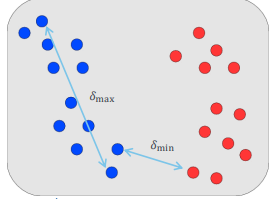
\includegraphics[scale=0.5]{assets/intrinsic_metric.png}
\end{center}
Higher is better. However, this biases towards one cluster per object.

\paragraph{Silhouette Coefficient}: $s(i)$ for object $x_i$. It uses several components
\begin{itemize}
  \item Average distance to all other objects in same cluster $\omega$
  \[a(i) = \sum_{x\in \omega, x \neq x_i} \frac{1}{|\omega| -1}\delta(x_i,x)\]
  \item Average distance to some other cluster $\omega'$
  \[d(i,\omega') = \sum_{x\in\omega'}\frac{1}{|\omega'|}\delta(x_i,x)\]
  \item Average distance to closest other cluster
  \[b(i) = \min_{\omega'\in\Omega, \omega'\neq \omega} d(i,\omega')\]
\end{itemize}
So the Silhouette coefficient is
\[s(i) = \frac{b(i)-a(i)}{\max(a(i),b(i))}\]

with
\[-1 \leq s(i) \leq 1\]
A value close to one implies $b(i)$ is much larger than $a(i)$. Value closer to -1 represents the opposite.

The aggregate would be the \textbf{average silhouette coefficient} would be 
\[\frac{1}{N}\sum s(i)\]

\subsubsection{Extrinsic Metrics}
We are given external ground truth of categories
\[C = \{c_i,...,c_J\}\]

Idea: compare $\Omega$ and $C$

We define $n_j^{(i)} := $number of objects from $c_i$ clustered into $\omega_j$

\paragraph{Purity }: Ratio of strongest represented category
\[Purity(\omega_j) = \frac{1}{|\omega_j|}\cdot \max_{i=1,...,J}n_j^{(i)}\]

Aggregate over all clusters
\[Purity(\Omega) = \sum_{j = 1}^{K}\frac{|\omega_j|}{N}Purity(\omega_j)\]
\begin{center}
  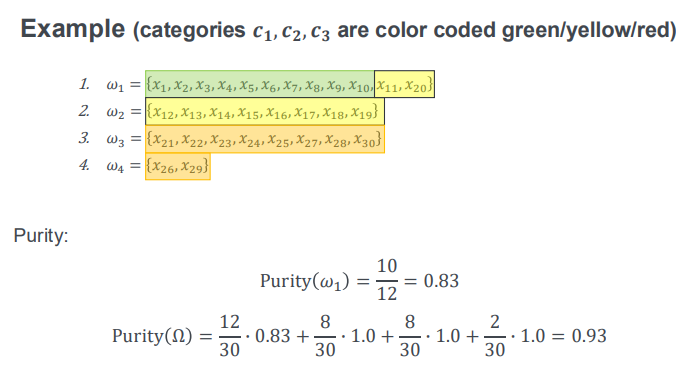
\includegraphics[scale=0.5]{assets/extrinsic_purity.png}
\end{center}

\paragraph{Mutual Information}: Mutual agreement between clusters and categories

\[MI(\Omega) = \frac{1}{N}\sum_{j=1}^{K}\sum_{i=1}^{J}n_j^{(i)}\cdot \log \frac{n_j^{(i)}\cdot N}{\sum_{m=1}^{J}n_j^{(m)}\sum_{l=1}^{K}n_j^{(i)}}\]

\paragraph{Rand Index}

For any pair of points $(x_a, x_b)$, we distinguish:

\begin{itemize}
    \item $ss$: same category, same cluster (agreement)
    \item $dd$: different category, different cluster (agreement)
    \item $sd$: same category, different cluster (disagreement)
    \item $ds$: different category, same cluster (disagreement)
\end{itemize}

\[
I_{\text{Rand}}(\Omega) =
\frac{ss + dd}{ss + dd + sd + ds}
\]

\paragraph{Interpretation}

\begin{itemize}
    \item $I_{\text{Rand}} = 1$: perfect agreement
    \item $I_{\text{Rand}} = 0$: complete disagreement
    \item Measures fraction of correctly decided pairs
\end{itemize}
Example:
\begin{center}
  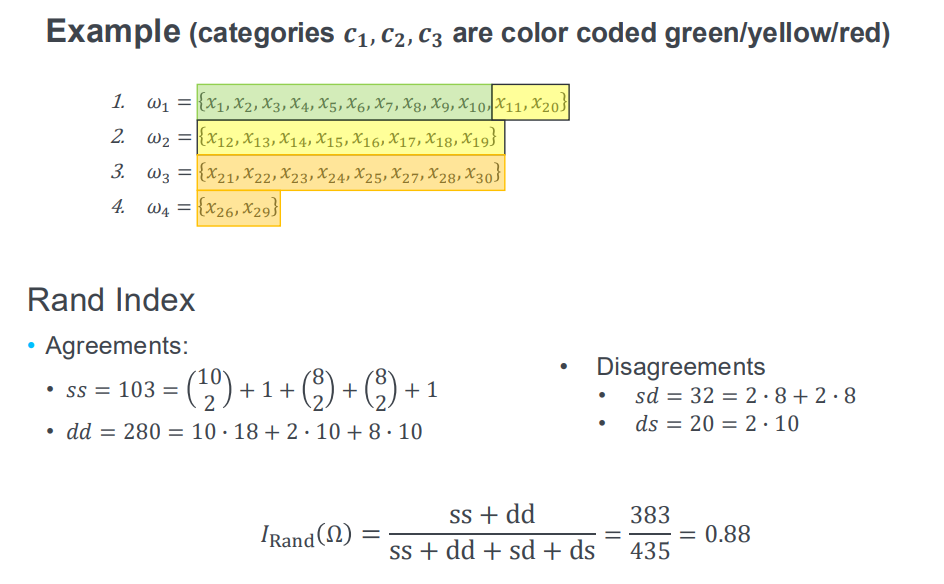
\includegraphics[scale=0.5]{assets/extrinsic_rand_index.png}
\end{center}

\subsection{Loss Function vs Evaluation Metric}
Don't confuse them! An evaluation metric is easy to understand, task specific truth that most humans find correct. A loss function is algorithm specific, complex and guides the algorithm to find the right solution.

\subsection{K-Means}
It's a general clustering algorithm. 

Parameters
\begin{itemize}
  \item K: Number of clusters
  \item Initial random seed
\end{itemize}

Given input data $\{x_i\}_{i=1}^N, x_i \in \mathbb{R}^d$ and $d,K \in \mathbb{N}$
\begin{algorithm}
Choose randomly K cluster centroid seeds $Z = {z_i | z_i \in \mathbb{R}^d}_{i=1}^K$\\

repeat\{\\
\quad  for all objects x. assign x to cluster $\omega_i$ with minimal $\delta(x,z_i)$\\
\quad  For all clusters $\omega_i$ compute centroid $z_i = \frac{1}{|\omega_i|}\sum_{x\in\omega_i}x$\\
\} repeat until centroids do not change\\
\end{algorithm}

It's really easy, decently quick (O(n) for each iterations, usually done after 5-10 iterations).

However, susceptible to noise and outliers. Clusters always have convex form. $k$ is sometimes hard to compute. Dependant on initial partition.


\subsubsection{Evaluate Quality}
Try different seeds and then evaluate quality for the best quality.

\begin{itemize}
  \item Dunn Index
  \item Residual Sum of Squares
  \[RSS(\Omega) = \sum_{j=1}^{K}\sum_{x\in\omega_j} \delta(x,z_j)^2\]
\end{itemize}

\subsubsection{Variations}
\begin{itemize}
  \item (Random) Seed: Furthest Points/ Furthest modified points
  \item Stop Criterion: Small changes of the centroids. Fixed number of iterations
  \item K-Medioid: Non-standard metrics (string similarity)
\end{itemize}

\subsubsection{Choice of K}
You have to have \textbf{some} knowledge about the data. More clusters always equates to less RSS, but it isn't always advantageous to have more clusters.

\subsubsection{Problematic Configurations}
\begin{center}
  \begin{tabular}{|c|c|}
    \hline
    Problem & Solution \\
    \hline
    Outliers & Remove and treat separately\\
    \hline
    Empty Clusters & Split large cluster\\
    \hline
    Non-spheric shapes & Cannot be handled \\
    \hline
  \end{tabular}
\end{center}\section{Expectation Maximization}

\textbf{Idea:} Assume that data is produced by a parameterized probability distribution.

\begin{center}
  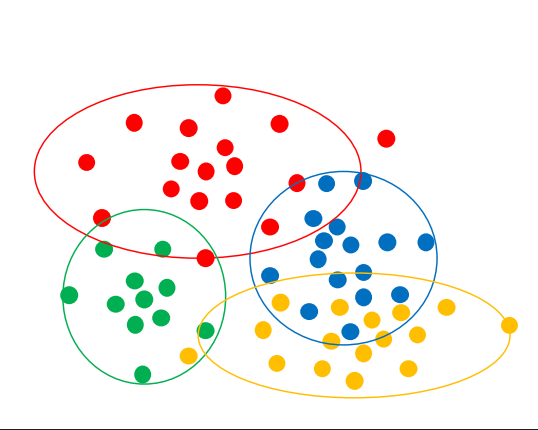
\includegraphics[scale=0.6]{assets/expectation_maximization.png}
\end{center}

The issue arises when we do not know the distributions and can only observe the raw data.

\begin{center}
  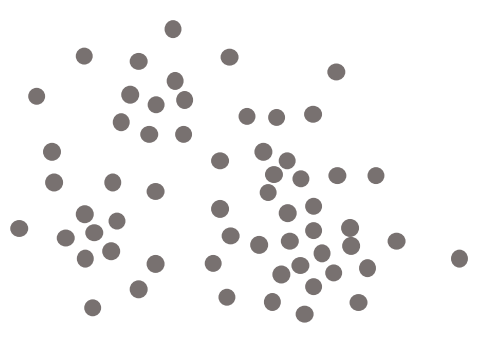
\includegraphics[scale=0.6]{assets/expectation_maximization_raw.png}
\end{center}

\textbf{Expectation Maximization (EM)} is a general clustering algorithm with a probabilistic
approach and soft cluster assignment. It is a further generalization of K-Means.

\paragraph{Parameters:}
\begin{itemize}
  \item $K$: Number of clusters
  \item Initial random seed
  \item Model for the distribution
\end{itemize}

\paragraph{Refresher on probabilistic distributions:}
A probability density function (PDF) $f(x)$ satisfies:
\[
  \int_{\Omega} f(x)\,dx = 1
\]
The cumulative distribution function (CDF) is defined as:
\[
  F(x) = P(X \leq x) = \int_{-\infty}^{x} f(t)\,dt
\]
For multiple dimensions:
\[
  F(x_1,\dots,x_n)
  = P(X_1 \leq x_1,\,\dots,\,X_n \leq x_n)
  = \int_{-\infty}^{x_1}\cdots\int_{-\infty}^{x_n}
    f(t_1,\dots,t_n)\,dt_n\cdots dt_1
\]

% -------------------------------------------------------
\subsection{Gaussian Models of Individual Distributions}

\subsubsection{Univariate Normal Distribution}
\[
  f(x) = \frac{1}{\sigma\sqrt{2\pi}}\,
         \exp\!\left(-\frac{(x-\mu)^2}{2\sigma^2}\right)
\]
where $\mu$ is the mean and $\sigma$ is the standard deviation.

\subsubsection{Multivariate Normal Distribution}
For a $d$-dimensional random vector $\mathbf{x}$, the density is:
\[
  f(\mathbf{x})
  = \frac{1}{(2\pi)^{d/2}|\Sigma|^{1/2}}\,
    \exp\!\left(-\frac{1}{2}(\mathbf{x}-\boldsymbol{\mu})^T
    \Sigma^{-1}(\mathbf{x}-\boldsymbol{\mu})\right)
\]
where $\boldsymbol{\mu}$ is the mean vector and $\Sigma$ is the covariance matrix.
The scalar standard deviation $\sigma$ is simply replaced by $\Sigma$.

% -------------------------------------------------------
\subsection{Model Estimation}

\paragraph{Maximum Likelihood Estimation (MLE):}
Given a dataset $X = \{x_1, \dots, x_n\}$, the \textbf{log-likelihood} is the logarithm of the
probability of observing the data under parameters $\theta$:
\[
  \log L(\theta \mid X)
  = \log\!\left(\prod_{x_i \in X} P(x_i \mid \theta)\right)
  = \sum_{x_i \in X} \log P(x_i \mid \theta)
\]
We take the logarithm because it converts the product into a sum, which is numerically stable
and easier to differentiate. Maximizing $\log L$ is equivalent to maximizing $L$ since $\log$
is monotonically increasing.

\medskip\noindent
Maximizing the log-likelihood yields the MLE estimators:

\begin{itemize}
  \item \textbf{1-dimensional case:}
  \[
    \hat{\mu} = \frac{1}{n}\sum_{i=1}^{n} x_i
    \qquad
    \hat{\sigma}^2 = \frac{1}{n}\sum_{i=1}^{n}(x_i - \hat{\mu})^2
  \]
  \item \textbf{$d$-dimensional case:}
  \[
    \hat{\boldsymbol{\mu}} = \frac{1}{n}\sum_{i=1}^{n} \mathbf{x}_i
    \qquad
    \hat{\Sigma} = \frac{1}{n}\sum_{i=1}^{n}
                  (\mathbf{x}_i - \hat{\boldsymbol{\mu}})
                  (\mathbf{x}_i - \hat{\boldsymbol{\mu}})^T
  \]
\end{itemize}

\noindent
Note: The MLE for variance uses $\tfrac{1}{n}$ and is a \emph{biased} estimator.
The unbiased sample variance uses $\tfrac{1}{n-1}$ (Bessel's correction), but in the
context of EM and MLE we use $\tfrac{1}{n}$.

\medskip\noindent
The computation above assumes we know which object belongs to each cluster. Without
cluster assignments, this is simply parameter estimation for a \emph{single} Gaussian
fitted to all the data — not a mixture. We need the EM algorithm to handle the unknown
cluster memberships.

% -------------------------------------------------------
\subsection{Cluster Assignment}

\paragraph{Assumption — Independently and Identically Distributed (i.i.d.):}
A dataset is i.i.d.\ if every observation $x_i$ is drawn independently from the same
underlying probability distribution. \emph{Independent} means the value of one observation
does not affect any other; \emph{identically distributed} means all observations follow the
same distribution with the same parameters. This lets us write the joint likelihood as a
simple product: $P(X \mid \theta) = \prod_{i} P(x_i \mid \theta)$.

\medskip\noindent
For each object $x_i \in X$ we model \textbf{latent variables} $z_{ij}$ indicating the
probability that $x_i$ belongs to cluster $\omega_j$. The algorithm alternates two steps
until convergence:

\begin{itemize}
  \item \textbf{E-step (Expectation):} Given the current model parameters $\theta$,
        compute the expected values of the latent variables $z_{ij}$. This yields the
        probability that object $x_i$ belongs to cluster $\omega_j$ under the current
        model.
  \item \textbf{M-step (Maximization):} Given the current estimates of the latent
        variables $z_{ij}$, update the model parameters $\theta$ by maximizing the
        expected log-likelihood.
  \begin{center}
    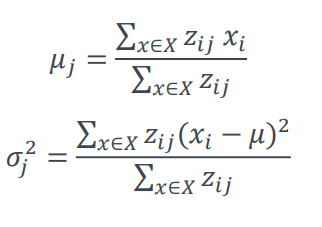
\includegraphics[scale=0.5]{assets/expected_maximization_formula.png}
  \end{center}
\end{itemize}

\subsubsection{Problem: Initialization}
The E-step requires model parameters $\theta$ to estimate the latent variables, while the
M-step requires latent variable estimates to update $\theta$. This circular dependency
means we must initialize $\theta$ before the first E-step, either randomly, via a
heuristic (e.g.\ running K-Means first), or by another method.

\subsubsection{Example}
By varying the parameters of the Gaussian components we can observe how the cluster
assignments change.

\begin{center}
  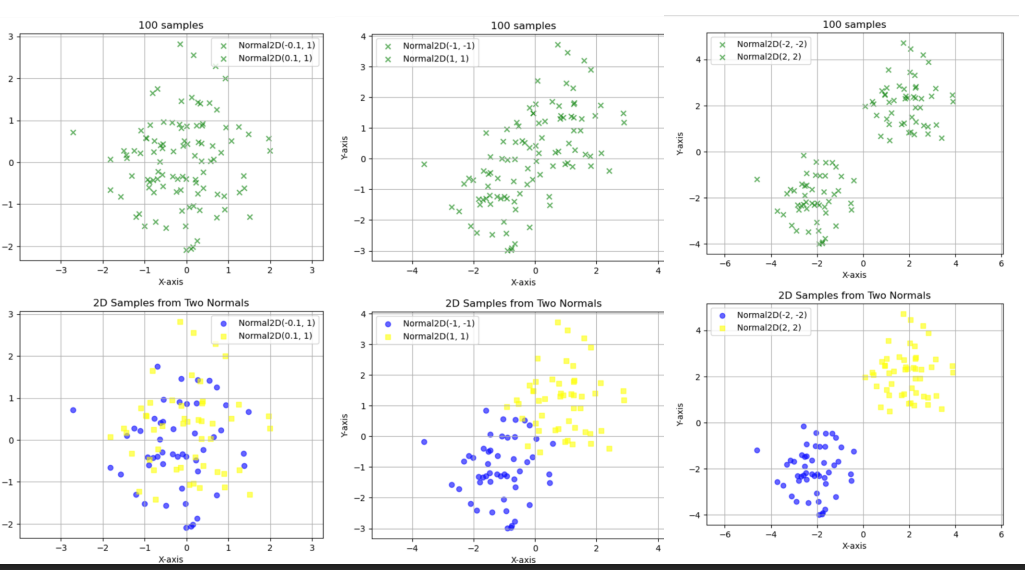
\includegraphics[scale=0.5]{assets/expectation_maximization_separation.png}
\end{center}
\section{Linear Regression}

\subsection{Interpolation}
Given a set of data points, find a polynomial that passes through all of them.

\subsubsection{Lagrange Interpolation}
\[
  \hat{f}(x) = \sum_{i=1}^{n} y_i \prod_{\substack{k=1\\k\neq i}}^{n} \frac{x - x_k}{x_i - x_k}
\]
\begin{itemize}
  \item Passes through every data point exactly
  \item Degree equals the number of data points minus one
  \item Very sensitive to outliers
\end{itemize}

\subsubsection{Piecewise Linear Interpolation}
Connect consecutive data points with straight lines.
\begin{itemize}
  \item Simple and fast
  \item Not smooth (sharp corners at data points)
  \item Sensitive to outliers
\end{itemize}

\subsubsection{Spline Interpolation}
Fit smooth polynomial pieces between data points, requiring the derivative to be
continuous at each interior point $x_i$:
\[
  \forall\, i \in \{2,\dots,n-1\}:\quad
  \lim_{\epsilon \to 0}\hat{f}'(x_i - \epsilon)
  = \lim_{\epsilon \to 0}\hat{f}'(x_i + \epsilon)
\]
\begin{itemize}
  \item Smooth transitions between segments
  \item Overly complex model $\Rightarrow$ tends to overfit outliers
\end{itemize}

\begin{center}
  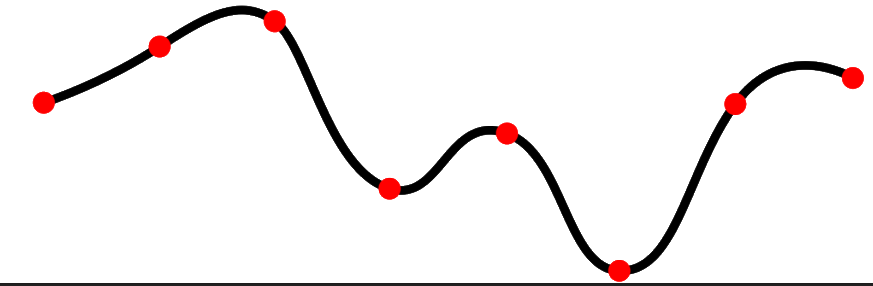
\includegraphics[scale=0.5]{assets/spline_interpolation.png}
\end{center}

% ----------------------------------------------------------------
\subsection{Regression}
Unlike interpolation, regression does \emph{not} require the function to hit every point.
Instead it finds the best-fitting function while tolerating noise.

We assume data is generated by a linear function with some noise $\epsilon$:
\[
  f(x) = \beta_1 x + \beta_0 + \epsilon
\]

\begin{center}
  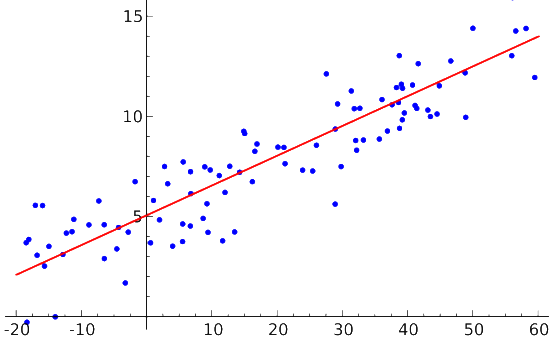
\includegraphics[scale=0.5]{assets/linear_regression.png}
\end{center}

\begin{itemize}
  \item Differences between predicted and actual values are called \textbf{residuals}
  \item Predictor variables ($x$) are also called \textbf{input variables}
\end{itemize}

\subsubsection{Variants}
\begin{itemize}
  \item \textbf{Simple linear regression:} one predictor $x_i$, one response $y_i$
  \item \textbf{Multiple linear regression:} multiple predictors
        $\mathbf{x}_i = (x_{i,1},\dots,x_{i,d})$, one response $y_i$
  \item \textbf{Multivariate linear regression:} multiple predictors
        \emph{and} multiple response variables
\end{itemize}

% ----------------------------------------------------------------
\subsubsection{Multiple Linear Regression}

\textbf{Goal:} estimate unknown parameters $\beta = (\beta_0,\dots,\beta_d)^T$,
assess their relevance, and estimate the error variance.

\paragraph{Scalar form:}
\[
  y_i = \beta_0 + \beta_1 x_{i,1} + \dots + \beta_d x_{i,d} + \epsilon_i
\]

\paragraph{Vector form:}
\[
  y_i = \bar{x}_i^T \beta + \epsilon_i
\]
\[
\begin{cases}
  \bar{x}_i = (1,\, x_{i,1},\dots, x_{i,d})^T \in \mathbb{R}^{d+1} \\
  \beta      = (\beta_0,\dots,\beta_d)^T       \in \mathbb{R}^{d+1} \\
  \epsilon   = (\epsilon_1,\dots,\epsilon_n)^T \in \mathbb{R}^{n}
\end{cases}
\]

\paragraph{Matrix form:}
\[
  \mathbf{y} = X\beta + \epsilon
  \qquad\text{where}\qquad
  X =
  \begin{pmatrix}
    \bar{x}_1^T \\
    \vdots \\
    \bar{x}_n^T
  \end{pmatrix}
  \in \mathbb{R}^{n\times(d+1)}
\]

\paragraph{Optimization objective:}
Find $\hat{\beta}$ that minimizes the sum of squared residuals (\textbf{least squares}):
\[
  L^{ls}(\beta)
  = \|\epsilon(\beta)\|^2
  = \|y - X\beta\|^2
  = (y - X\beta)^T(y - X\beta)
\]

\paragraph{Determine Extreme Value}: We equalize the derivative to zero. This closed-form solution exists as long as $X^TX$ is invertible

\[-2(y-X\beta)^TX = 0^T_d \Rightarrow 0^T_d = X^TX\beta - X^Ty \Rightarrow \hat{\beta}^{ls} = (X^TX)^{-1}X^Ty\]

This is the theoretical solution, but not commonly used because of inefficiency and computationally unstable. We use stochastic gradient descent to find where $X^TX\beta - X^T y$ is zero in all its components
\paragraph{Beyond Linear Input}
Linear regression is called ``linear'' not because the input has to be linear,
but because the model is linear in the \textbf{parameters} $\beta$.
This means we are free to transform the raw inputs into something non-linear first,
and then fit a regular linear model on top. Think of it as: instead of feeding the
model plain $x$, you can square it, apply a Gaussian, etc. and
\textit{then} fit a line through the result.

We replace the inputs ($x_i \in \mathbb{R}^d$) with non-linear features
$\phi(x_i) \in \mathbb{R}^k$, so that

\[
    y = \sum_{j=1}^{k} \phi_j(x)\,\beta_j + \epsilon \;=\; \phi(x)^T\beta + \epsilon
\]

The catch: we still have to choose what $\phi$ looks like -- that's the
``guessing'' part.

% -------------------------------------------------------------------
\paragraph{Example: Polynomial features}
The simplest non-linear trick. Instead of using just $x$, you add $x^2$, $x^3$,
\ldots as extra input columns. The model stays linear in $\beta$, but can now
fit curved relationships.

\begin{center}
  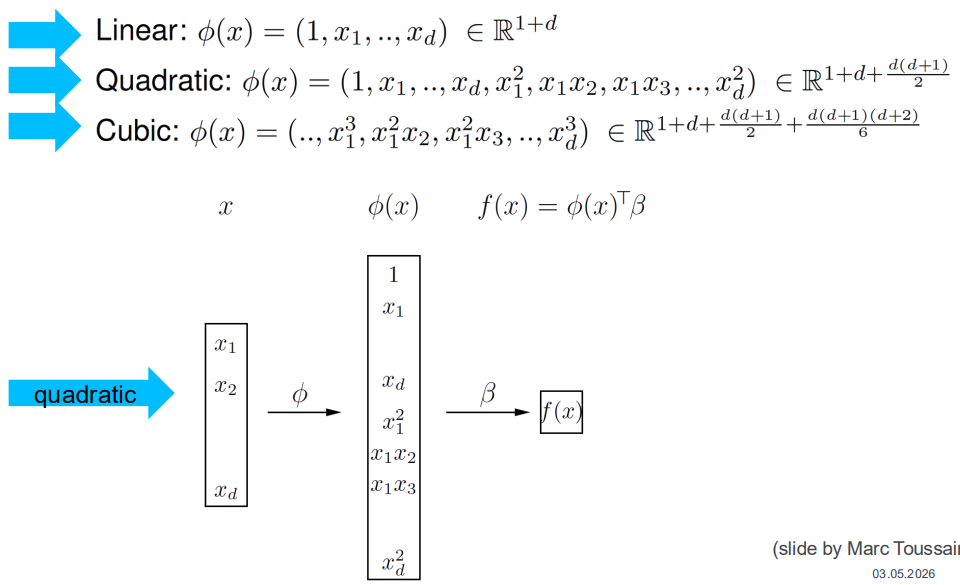
\includegraphics[scale=0.5]{assets/polynomial_feature_regression.png}
\end{center}

% -------------------------------------------------------------------
\paragraph{Example: Piece-wise features (in 1D)}
Instead of one global curve, we chop the $x$-axis into intervals
(``pieces'') and fit something simple inside each piece.
We use the notation: $[\text{condition}] = 1$ if the condition is true, otherwise 0,
and $[t]_+ = t$ if $t > 0$, otherwise 0(a ramp / ReLU).

\begin{itemize}
  \item \textbf{Piece-wise constant:} $\phi_j(x) = [\xi_j < x \leq \xi_{j+1}]$
        \hfill flat step inside each bin, because for a single point $x_i$, its prediction would be
        \[\sum_{j=1}^N \phi_j(x_i) \cdot w_j = w_j\]
        Because all the basis functions apart from $i$ return zero.
  \item \textbf{Piece-wise linear:} $\phi_j(x) = (1,\,x)^T[\xi_j < x \leq \xi_{j+1}]$
        \hfill a separate line in each bin (can jump at boundaries).
  \item \textbf{Continuous piece-wise linear:} $\phi_j(x) = [x - \xi_j]_+$
        (with $\phi_0(x)=x$) \hfill lines that are forced to connect at each knot.
\end{itemize}

\begin{center}
  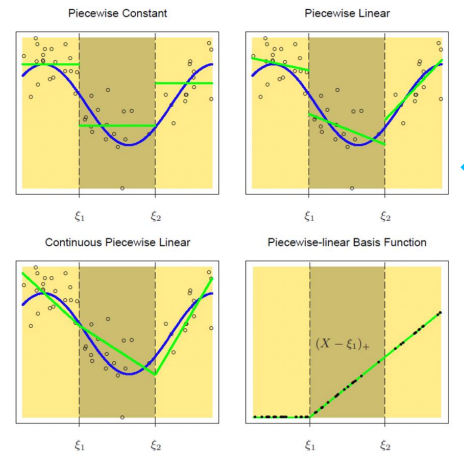
\includegraphics[scale=0.5]{assets/piecewise.png}
\end{center}

% -------------------------------------------------------------------
\paragraph{Example: Radial Basis Function (RBF)}
Pick a set of ``center'' points $\{c_j\}_{j=1}^{k}$ spread across your data.
Each feature just measures \textit{how close} $x$ is to one center using a
Gaussian bell-curve:

\[
    \phi_j(x) \;=\; b(x,\,c_j) \;=\; e^{-\frac{1}{2}\|x - c_j\|^2} \;\in [0,1]
\]

When $x$ is right on top of $c_j$ the feature is 1; the further away, the closer
to 0. So the model ends up as a weighted sum of bumps.

% ===================================================================
\subsection{Model Quality of Linear Regression}

% -------------------------------------------------------------------
\subsubsection{Mean vs Median}

\textbf{Mean regression} minimises the squared-error loss $\ell = \epsilon^T\epsilon$.\\
\textbf{Median regression} minimises the absolute-error loss
$\ell = \sum_i |\epsilon_i|$.

The squared loss punishes big errors \textit{a lot} (because it squares them),
so one extreme outlier can drag the whole fit away. The absolute loss treats
every unit of error equally, making it far more robust to weird data points.

\begin{center}
  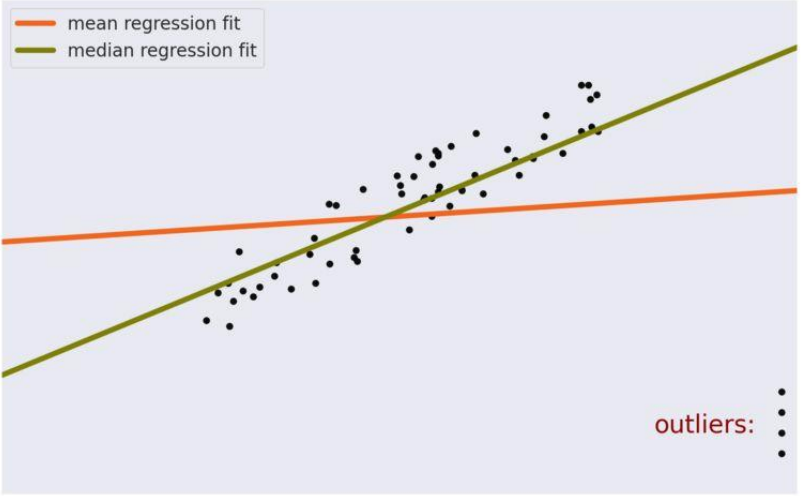
\includegraphics[scale=0.5]{assets/mean_vs_median_regression.png}
\end{center}

% -------------------------------------------------------------------
\subsubsection{The Hat Matrix}

The hat matrix $H = X(X^TX)^{-1}X^T$ is called that because it ``puts a hat''
on $y$:
\[
    \hat{y} = Hy
\]
It is the projection matrix that maps the observed $y$ onto the column space of
$X$ The issue is that $\hat{y}$ (our prediction) lives as a linear combination of the feature columns of $X$. This restricts $\hat{y}$ to a subspace. For that, we use this Hat matrix to project $y$ to the subspace of $\hat{y}$ Each diagonal entry $h_{ii}$ (called \textit{leverage}) tells you how much
observation $i$ can pull the regression line towards itself -- high leverage points are
potentially dangerous.

\begin{center}
  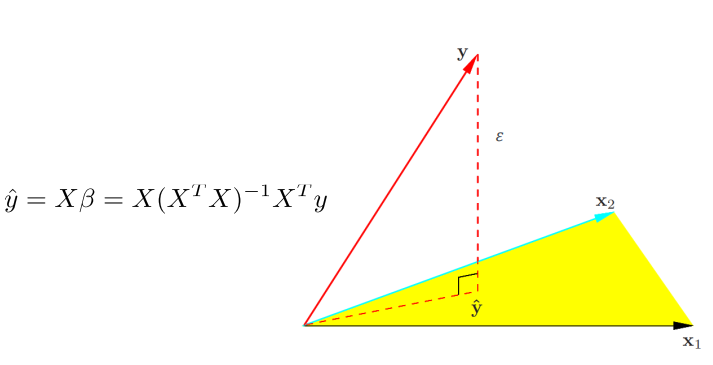
\includegraphics[scale=0.5]{assets/hat_matrix.png}
\end{center}

% -------------------------------------------------------------------
\subsubsection{Residuals}

Residuals are what's left over after the model does its best: $e_i = y_i - \hat{y}_i$.
If everything is fine they should look like \textit{random noise} -- no patterns.

\textbf{Tukey--Anscombe plot}: residuals $e_i$ vs fitted values $\hat{y}_i$.
Patterns in this plot signal problems:

\begin{itemize}
  \item Residuals grow linearly with $\hat{y}$ -- some systematic bias, wrong
        functional form.
  \item Residuals grow non-linearly with $\hat{y}$ -- the true relationship is
        curved and the model misses it.
  \item Two distinct clouds with different spread -- two sub-populations with
        different variances.
  \item A U-shape / arch -- a quadratic term is missing from the model.
\end{itemize}

% ===================================================================
\subsection{Investigating Model Assumptions}

For the standard theory to hold, we assume:

\begin{enumerate}
  \item Residuals are jointly normally distributed with $\mathbb{E}(\epsilon_i) = 0$
        and $\operatorname{Var}(\epsilon_i) = \sigma^2$ for all $i$.
        \textit{(Errors are centred and not huge on average.)}
  \item The variance $\sigma^2$ is the \textbf{same} for every observation
        (\textit{homoscedasticity}). \textit{(No observation is inherently
        noisier than another.)}
  \item All $x_i$ are observed \textbf{without noise}. \textit{(Only $y$ is
        noisy, not $x$.)}
  \item Errors are uncorrelated: $\operatorname{Cov}(\epsilon_i, \epsilon_j) = 0$
        for $i \neq j$. \textit{(One bad measurement doesn't infect the next.)}
\end{enumerate}

Under these assumptions, since $y_i = x_i^T\beta + \epsilon_i$ and $\beta,x$ are
exact, every $y_i$ has $\operatorname{Var}(y_i)=\sigma^2$.
If the residuals don't have mean zero, your model is missing something.

% ===================================================================
\subsection{Goals of Linear Regression Analysis}

\begin{enumerate}

  % --- Goal 1 -------------------------------------------------------
  \item \textbf{Good fit}: Small training error.

  \paragraph{Estimator Variance}
  Given $\epsilon \sim \mathcal{N}(0,\sigma^2)$ we get
  $y \sim \mathcal{N}(X\beta,\,\sigma^2 I)$, and $\hat{\beta}$ is itself
  normally distributed:
  \[
      \hat{\beta} \sim \mathcal{N}\!\left(\beta,\;\sigma^2(X^TX)^{-1}\right)
  \]
  More data $\Rightarrow$ $(X^TX)^{-1}$ shrinks $\Rightarrow$ $\hat{\beta}$
  wobbles less around the truth.

  % --- Goal 2 -------------------------------------------------------
  \item \textbf{Good prediction}: Small test error.

  \paragraph{Overfitting and generalisation}
  A more expressive model always reduces training error, but it starts memorising
  the noise in the training data instead of the true signal -- it then performs
  poorly on new data.

  \paragraph{Bias--Variance decomposition}
  Let $D$ be the training set, $\hat{f}=\hat{f}(x;D)$ our estimate, and
  $f$ the true function. Using
  $\operatorname{Var}[X] = \mathbb{E}[X^2] - \mathbb{E}[X]^2$,
  $\mathbb{E}[\epsilon]=0$, $\mathbb{E}[\epsilon^2]=\sigma^2$, and
  $y = f + \epsilon$, we can show:

  \[
      \mathbb{E}\!\left[(y - \hat{f})^2\right]
      \;=\;
      \underbrace{\sigma^2}_{\text{noise}}
      \;+\;
      \underbrace{\operatorname{Var}[\hat{f}]}_{\text{variance}}
      \;+\;
      \underbrace{\operatorname{Bias}[\hat{f}]^2}_{\text{bias}}
  \]

  \textit{Simple models}: high bias (they miss the true shape), low variance
  (they don't change much with different training sets).\\
  \textit{Complex models}: low bias, high variance (they overfit the noise).
  You want the sweet spot in the middle.

  \begin{center}
    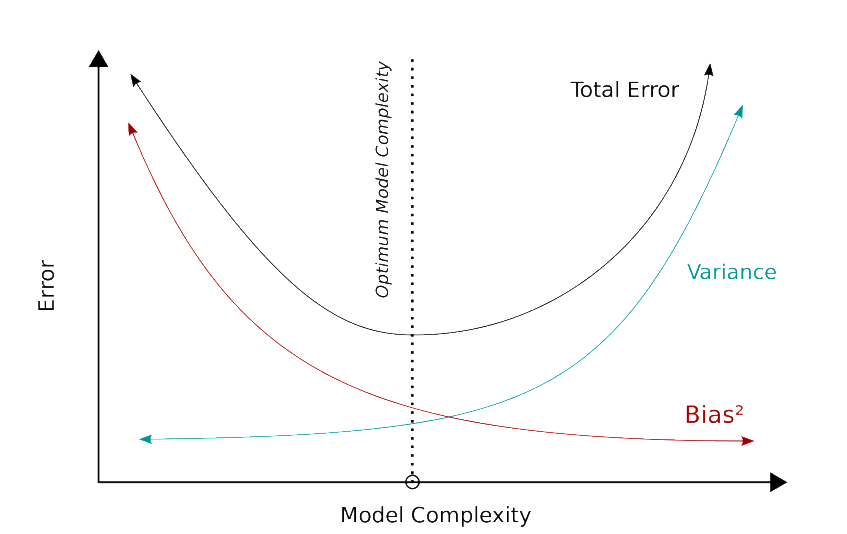
\includegraphics[scale=0.5]{assets/bias_variance_tradeoff.png}
  \end{center}

  % --- Goal 3 -------------------------------------------------------
  \item \textbf{Good parameter estimates}: What are the actual $\beta_j$ values?

  With one predictor $y = \beta_0 + \beta_1 x$, standardise everything to
  zero mean, unit variance:
  \[
      x^* = \frac{x - \bar{x}}{\sigma_x}, \qquad
      y^* = \frac{y - \bar{y}}{\sigma_y}
  \]
  After standardisation $\beta_0^* = 0$, and the slope equals the
  \textbf{Pearson correlation}:
  \[
      \rho_{x,y}
      \;=\;
      \beta_1^*
      \;=\;
      \frac{1}{n}\sum_{i=1}^{n} x_i^* y_i^*
      \;=\;
      \beta_1\,\frac{\sigma_x}{\sigma_y}
  \]
  So the standardised slope \textit{is} the correlation -- it tells you the
  strength and direction of the linear relationship, on a $[-1,1]$ scale.

  % --- Goal 4 -------------------------------------------------------
  \item \textbf{Uncertainties and significance}: Are any predictors actually
  doing something useful?

  For each predictor $j$ (corresponding to variable $X_j$) we run a hypothesis test:\\
  \quad $H_{0,j}$: $\beta_j = 0$ (this predictor has no effect)\\
  \quad $H_{A,j}$: $\beta_j \neq 0$ (it does have an effect)

  If we can reject $H_{0,j}$, predictor $j$ is statistically significant.

\end{enumerate}

% ===================================================================
\subsection{Reducing Model Complexity}

\subsubsection{Subset Selection}

Least-squares estimates have two practical problems:

\begin{enumerate}
  \item \textbf{Prediction accuracy}: Low bias but potentially huge variance.
        Shrinking or zeroing some $\beta_j$ can actually \textit{improve}
        test error even though training error goes up slightly.
  \item \textbf{Interpretation}: With dozens of predictors, the model is a mess
        to explain. Keeping only the strongest predictors gives a cleaner story.
\end{enumerate}

Fewer variables $=$ easier to interpret, often better generalisation.

% -------------------------------------------------------------------
\subsubsection{Ridge Regression (L2)}

Ridge adds a penalty on the size of $\beta$ to prevent it from blowing up.
Instead of minimising squared error freely, we force
$\sum_{j=1}^d \beta_j^2 \leq t$ for some budget $t$:

\[
    \hat{\beta}^{\text{ridge}}
    \;=\;
    \arg\min_{\beta}
    \sum_{i=1}^{n}
    \left(y_i - \beta_0 - \sum_{j=1}^{d} x_{i,j}\,\beta_j\right)^2
    \quad\text{subject to}\quad
    \sum_{j=1}^{d} \beta_j^2 \leq t
\]

Equivalently, via a Lagrange multiplier $\lambda \geq 0$:

\[
    \hat{\beta}^{\text{ridge}}
    \;=\;
    \arg\min_{\beta}
    \left[
    \sum_{i=1}^{n}
    \left(y_i - \beta_0 - \sum_{j=1}^{d} x_{i,j}\,\beta_j\right)^2
    +\,\lambda\sum_{j=1}^{d}\beta_j^2
    \right]
\]

\textbf{Note:} $\arg\min_\beta$ refers to finding the $\beta$ values which minimize the expression within the brackets. The first part is the Residual Sum of Squares, and the second part is our Penalty.

Larger $\lambda$ $\Rightarrow$ stronger shrinkage $\Rightarrow$ simpler model.
Setting $\lambda=0$ recovers ordinary least squares.

\subsubsection{Lasso Regression (L1)}
Instead of the Penalty being $\lambda\sum_{j=1}^{d}\beta_j^2$, it is $\lambda\sum_{j=1}^{d}|\beta_j|$

So the updated formula is
\[
    \hat{\beta}^{\text{lasso}}
    \;=\;
    \arg\min_{\beta}
    \left[
    \sum_{i=1}^{n}
    \left(y_i - \beta_0 - \sum_{j=1}^{d} x_{i,j}\,\beta_j\right)^2
    +\,\lambda\sum_{j=1}^{d}|\beta_j|
    \right]
\]

The Lasso has a diamond shape, so it is more biased for coefficients to be equal zero. It produces more sparcity. Ridge's coefficients almost never equal zero, it has a circle shape. Every feature stays in the model, but their influence is minimized

\begin{center}
  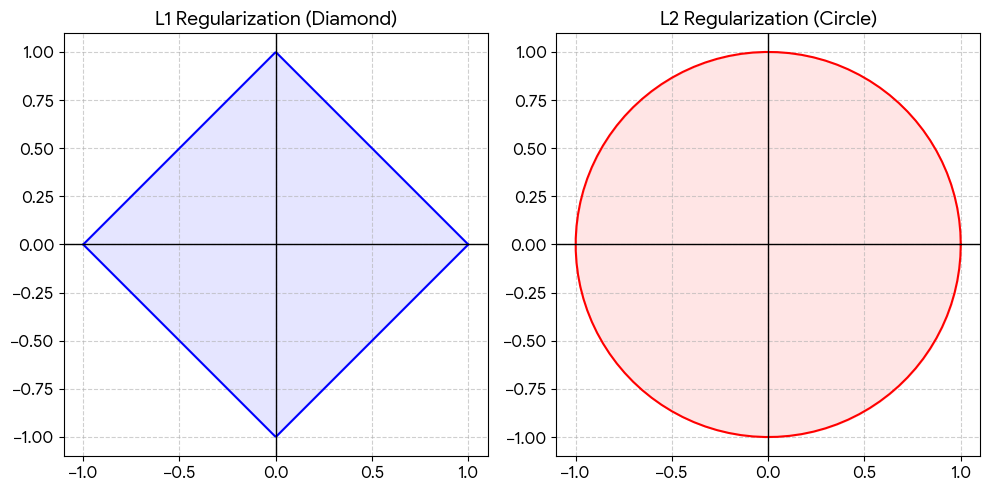
\includegraphics[scale=0.5]{assets/lasso_vs_ridge.png}
\end{center}

\subsubsection{Choosing hyperparameter $\lambda$}
So the lambda symbolizes how strong the penalty is. It controls the tradeoff between fitting the data well and keeping the model simple.

For $\lambda = 0$ we will always have a lower training data error, but we need to test the generalization error

\paragraph{k-fold cross validation}
\begin{center}
  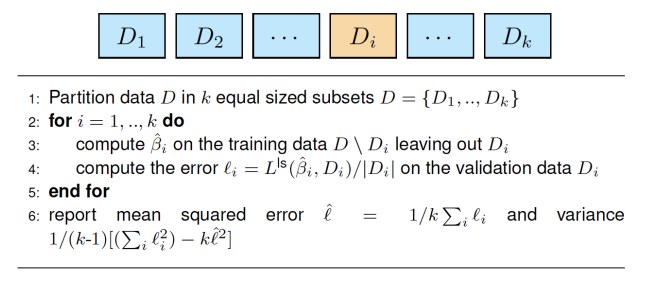
\includegraphics[scale=0.5]{assets/k_fold_cross_validation.png}

  Choose the $\lambda$ for which $\hat{l}$ is smallest.

\end{center}


\section{Classification}

\subsection{Ground Truth Classifier}
Given objects $x_i \in X$ described by $m$ attributes from a set of domains $\mathcal{A} = \{A_1, \dots, A_m\}$, such that:
\[ \forall i: x_i = (x_{i,1}, \dots, x_{i,m})^T \]
with $x_{i,k} \in A_k$.

We also define our set of target categories (classes) as $Y = \{l_1, \dots, l_k\}$. 
 \[ f: X \to Y \]

Our objective is to find the best possible approximation of $f$, denoted as $\hat{f}$. To achieve this, we restrict our search to a predefined hypothesis space (a family of functions) $\mathcal{F}$.

\subsection{Defining the Task of Learning a Classifier}
Given a dataset $\mathcal{D}$ containing $n$ i.i.d. samples, $\mathcal{D} = \{(x_1, y_1), \dots, (x_n, y_n)\} \sim X \times Y$, where each object $x_i$ consists of $m$ attributes and an observed category label $y_i \in Y$.

Given a parameterized function family $\mathcal{F}$, our goal is to find an optimal function $\hat{f}_{\theta} \in \mathcal{F}$ (where $\hat{f}_{\theta}: A_1 \times \dots \times A_m \to Y$) that minimizes the empirical risk.

\[\hat{f}_{\theta} = \arg\min_{\tilde{f}\in F }\sum_{i=1,...,n}l(\tilde{f}(x_i),y_i)\]

\subsubsection{Empirical Risk Minimization (ERM)}
While we ideally want to minimize the expected risk (true loss over the entire data distribution):
\[ R(f) = \mathbb{E}_{(x,y) \sim P(X,Y)} [l(\hat{f}_{\theta}(x), y)] \]
we do not have access to the true joint probability distribution $P(X,Y)$. By the Law of Large Numbers, we can approximate the expected loss using the average loss over our training data $\mathcal{D}$. This core machine learning paradigm is known as \textbf{Empirical Risk Minimization}:
\[ \arg\min_{\theta} \frac{1}{n} \sum_{i=1}^{n} l(\hat{f}_{\theta}(x_i), y_i) \overbrace{\Rightarrow}^{\text{LLN}} \arg\min_\theta \mathbb{E}[l(\hat{f}_\theta (x), y)]\]

In summary, engineering a machine learning pipeline consists of four pillars:
\begin{enumerate}
  \item \textbf{Model Design:} Define the hypothesis space $\hat{f}_{\theta}$.
  \item \textbf{Data Pipeline:} Collect, clean, and augment data $(x_i, y_i)$.
  \item \textbf{Loss Function:} Design a suitable objective function $l$.
  \item \textbf{Optimization Method:} Select an algorithm to solve $\arg\min_{\theta}$.
\end{enumerate}

\section{Validation and Evaluation}
A strict separation between training and testing data is essential to assess generalization. 

\begin{itemize}
    \item \textbf{K-Fold Cross-Validation:} The training data can be split into folds for internal validation and hyperparameter tuning, but it must never contain or interact with the test data.
    \item \textbf{Test Data:} Reserved exclusively for the final evaluation of the model's generalization capabilities.
\end{itemize}

\subsection{Combating Overfitting}
To effectively tune and evaluate models, the dataset should be split into three non-overlapping subsets:
\begin{enumerate}
    \item \textbf{Training Set:} Used to fit the model parameters ($\theta$) by minimizing the loss
    \item \textbf{Validation Set:} Used to evaluate performance during training and tune hyperparameters.
    \item \textbf{Test Set:} Used strictly for the final performance evaluation.
\end{enumerate}

\subsection{Evaluation Metrics for Classifiers}

\begin{center}
  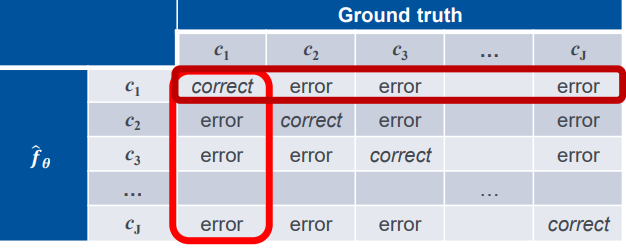
\includegraphics[scale=0.5]{assets/confusion_matrix.png}
\end{center}

Let $a_{ij}$ denote the number of elements belonging to class $c_j$ that were predicted as class $c_i$. We can define class-specific performance metrics:

\begin{enumerate}
  \item \textbf{Recall} $r(c_i)$: The ratio of correctly predicted objects in class $c_i$ out of all actual objects in $c_i$.
  \[ r(c_i) = \frac{a_{ii}}{\sum_{k=1}^{J} a_{ki}} \]
  
  \item \textbf{Precision} $p(c_i)$: The ratio of correctly predicted objects in class $c_i$ out of all objects predicted as $c_i$.
  \[ p(c_i) = \frac{a_{ii}}{\sum_{k=1}^{J} a_{ik}} \]
  
  \item \textbf{\texorpdfstring{$F_1$}{F1}-Score} $F_1(c_i)$: The harmonic mean of precision and recall.
  \[ F_1 = \frac{2 \cdot r(c_i) \cdot p(c_i)}{r(c_i) + p(c_i)} \]
\end{enumerate}

\subsubsection{Global Metric: Accuracy}
Accuracy measures the overall fraction of correct predictions across all $J$ categories.

\begin{center}
  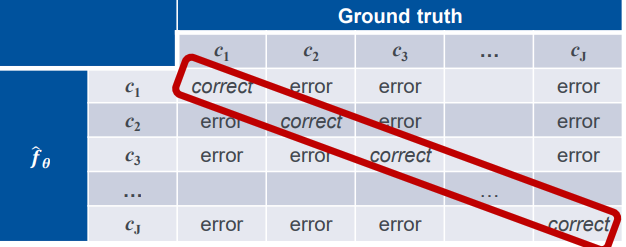
\includegraphics[scale=0.5]{assets/confusion_matrix_accuracy.png}
\end{center}

\[ \text{Accuracy} = \frac{\sum_{i=1}^{J} a_{ii}}{\sum_{i=1}^{J} \sum_{j=1}^{J} a_{ij}} \]

\subsubsection{Classification Errors}
In binary classification, errors are categorized as follows:
\begin{enumerate}
  \item \textbf{Type I Error (False Positive):} The model falsely predicts a positive condition for a negative instance.
  \item \textbf{Type II Error (False Negative):} The model falsely predicts a negative condition for a positive instance.
\end{enumerate}

\subsection{Data Leakage}
Data leakage occurs when information from outside the training dataset is inadvertently used to train the model. This causes the algorithm to create an overly optimistic performance baseline during validation, while failing to generalize to truly unseen data.

\section{Naïve Bayes}
\textit{Prerequisite Note: This method relies fundamentally on conditional probability and Bayes' Theorem.} This is covered in the first slides regarding Bayes Classification

\subsection{Bayes Classifier}
The objective is to make classification decisions probabilistically based on an observation vector $o = (x_1, \dots, x_m)$.

\begin{itemize}
  \item \textbf{Soft Classification:} Outputs the complete posterior probability distribution over all possible classes.
  \[ \hat{f}_{\text{soft}}(o) = P(c \mid o) \]
  \item \textbf{Hard Classification:} Predicts the single specific class that yields the highest posterior probability.
  \[ \hat{f}_{\text{hard}}(o) = \arg\max_{c \in C} P(c \mid o) \]
\end{itemize}

By applying Bayes' Theorem, the posterior probability is calculated as:
\[ P(c \mid o) = \frac{P(c) \cdot P(o \mid c)}{P(o)} = \frac{P(c) \cdot P(x_1, \dots, x_m \mid c)}{P(x_1, \dots, x_m)} \]

Where:
\begin{enumerate}
  \item $P(o)$: The \textbf{Evidence}. The marginal probability of the observation vector. It acts as a normalization constant and remains identical for all classes $c \in C$.
  \item $P(c)$: The \textbf{Prior}. The baseline probability of a category before observing any data attributes.
  \item $P(o \mid c)$: The \textbf{Likelihood}. The probability of observing features $o$ given that the object belongs to class $c$.
  \item $P(c \mid o)$: The \textbf{Posterior}. The updated probability that the observation belongs to class $c$ after evaluating its attributes.
\end{enumerate}

\subsection{Full (Non-Naïve) Bayes Classifier}
In a full Bayes framework, attributes and class labels are treated as mutually interdependent random variables. Modeling their full joint distribution requires tracking all complex combinations of dependencies.
\begin{center}
  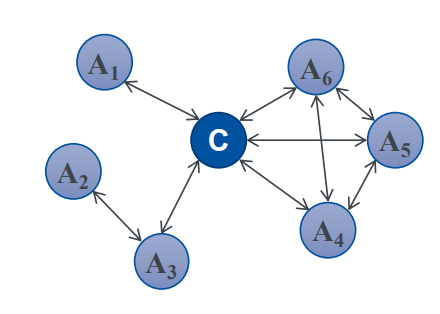
\includegraphics[scale=0.5]{assets/non_naive_bayes.png}
\end{center}

\subsection{Naïve Bayes Classifier}
The \textbf{Naïve Bayes assumption} radically simplifies calculations by assuming that all attributes are conditionally independent of each other, given the class label $c$.
\begin{center}
  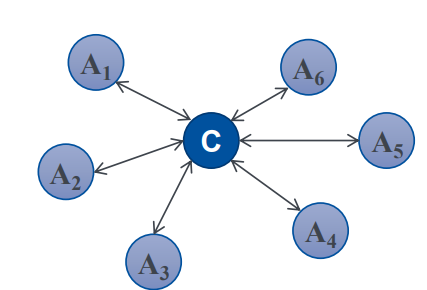
\includegraphics[scale=0.5]{assets/naive_bayes.png}
\end{center}

Using the chain rule of probability, the true likelihood expands exactly as:
\[ P(o \mid c) = P(x_1, \dots, x_m \mid c) = P(x_1 \mid x_2, \dots, x_m, c) \cdot P(x_2 \mid x_3, \dots, x_m, c) \dots P(x_m \mid c) \]

Applying the conditional independence assumption simplifies this long expression to a clean product of independent marginal likelihoods:
\[ P(x_1, \dots, x_m \mid c) \approx \prod_{j=1}^{m} P(x_j \mid c) \]

Substituting this approximation back into Bayes' Theorem yields the standard formulation for the Naïve Bayes model:
\[ P(c \mid x_1, \dots, x_m) \approx \frac{P(c)}{P(x_1, \dots, x_m)} \prod_{j=1}^{m} P(x_j \mid c) \]

\subsubsection{Smoothing for Naïve Bayes Classifier}
\paragraph{Laplace Smoothing}: The issue is that with the formula above, as soon as one of the $P(x_j|c) = 0$, the entire product is zero.

\[ P_{\text{Laplace}}(x_j = v \mid c_i) = \frac{|\{(x_1,\dots,x_m,c) \in O : x_j = v \land c = c_i\}| + 1}{|\{(x_1,\dots,x_m,c) \in O : c = c_i\}| + |V_j|} \]
\begin{quote}
\textbf{What it represents:} If a feature value never appears alongside class $c_i$ in the training data, its probability is 0. Because Naïve Bayes multiplies all probabilities together, a single zero makes the entire global probability 0. We add $+1$ to the numerator (and scale the denominator by $|V_j|$, the set of values for attribute $x_j$ ) to guarantee every feature retains a baseline chance of occurring.
\end{quote}

We can generalize this concept by substituting a custom parameter $\lambda$:
\paragraph{Generalized Additive Smoothing (Lidstone)}: 
\[ P_{\text{Lidstone}}(x_j = v \mid c_i) = \frac{|\{(x_1,\dots,x_m,c) \in O : x_j = v \land c = c_i\}| + \lambda}{|\{(x_1,\dots,x_m,c) \in O : c = c_i\}| + |V_j| \cdot \lambda} \]

\paragraph{Implementation Detail (Log-Transformation):}
Calculating probabilities directly via:
\[ P(c \mid x_1,\dots,x_m) \propto P(c) \cdot \prod_{j=1}^m P(x_j \mid c) \]
is numerically unstable on computers. Multiplying many values close to zero causes floating-point \textit{underflow} (rounding down to absolute 0). To stabilize this, we apply logarithms to turn multiplications into sums:
\[ \log P(c \mid x_1,\dots,x_m) \propto \log(P(c)) + \sum_{j=1}^{m} \log(P(x_j \mid c)) \]

\subsubsection{Handling Numerical (Continuous) Values}
\begin{quote}
\textbf{The Problem:} For continuous fields (like precise height or weight measurements), the probability of observing an exact scalar value is zero ($P(\text{weight} = 67.0000\dots) = 0$).
\end{quote}

To fix this, we replace discrete counts with continuous distributions. Let $X$ be a continuous random variable governed by a \textbf{probability density function} (PDF) $p(x) \in [0,\infty)$:
\[ P(a \leq x \leq b) = \int_{a}^b p(x) \, dx \in [0,1] \]
Its corresponding \textbf{cumulative probability distribution} (CDF) is defined as:
\[ F(y) = P(x \leq y) = \int_{-\infty}^y p(x) \, dx \in [0,1] \]

We assume continuous attributes follow a Gaussian (Normal) Distribution within each class:
\[ \mathcal{N}(x \mid \mu, \sigma^2) = p(x \mid \mu, \sigma^2) = \frac{1}{\sigma\sqrt{2\pi}} e^{-\frac{1}{2}\left(\frac{x-\mu}{\sigma}\right)^2} \]
We determine the parameters using Maximum-Likelihood Estimation (MLE):
\[ \mu_i = \frac{1}{n}\sum_{o}x_i, \quad \text{var}_i = \frac{1}{n-1}\sum_{o}(x_i-\mu_i)^2, \quad \sigma_i = \sqrt{\text{var}_i} \]

\begin{center}
  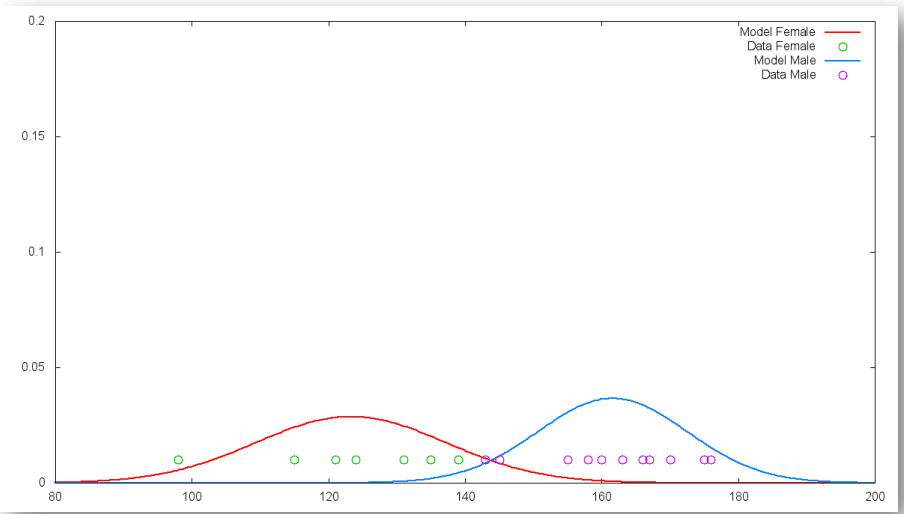
\includegraphics[scale=0.5]{assets/model_distribution_numeric_data.png}
  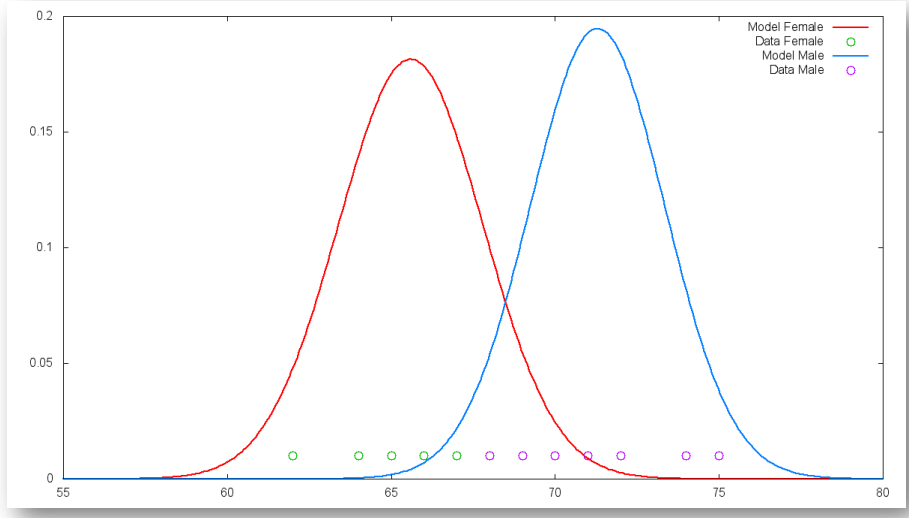
\includegraphics[scale=0.5]{assets/model_distribution_numeric_data_weight.png}
\end{center}

To utilize these continuous density functions for calculating class probabilities without getting 0, we evaluate a tiny interval around our target point $x$ using a small margin $\varepsilon$:
\[ P(\text{weight} = 67 \pm \varepsilon \mid c = f) \]
\begin{center}
  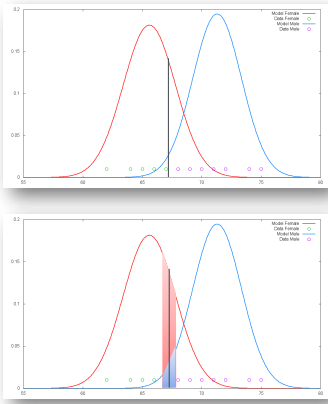
\includegraphics[scale=0.65]{assets/model_distribution_numeric_solution.png}
\end{center}


\section{Logistic Regression}
In Linear regression we predicted continous values, while here we predict discrete categories.

\subsection{Bayes Error \& Expected Prediction Error}
\begin{quote}
\textbf{What it represents:} The Expected Prediction Error (EPE) is a formal mathematical way of measuring the average penalty your model incurs for making incorrect predictions over a true data distribution.
\end{quote}

If we utilize a \textbf{Squared Error Loss} function for numerical predictions, the error is formulated as:
\[ EPE(\hat{f}) = E\left[(Y - \hat{f}(X))^2\right] = \int [y - \hat{f}(x)]^2 P(dx,dy) \]
Under this constraint, the absolute best mathematical prediction function matches the conditional mean:
\[ \hat{f}(x) = E(Y \mid X = x) \]

If we switch to an \textbf{Absolute Error Loss} function:
\[ EPE(\hat{f}) = E(|Y-\hat{f}(X)|) = \int |y-\hat{f}(x)| P(dx,dy) \]
The mathematically optimal prediction function matches the conditional median:
\[ \hat{f}(x) = \text{median}(Y \mid X = x) \]
\textbf{Note:} Absolute loss is rarely used during training optimization because the absolute value brackets $| \dots |$ are not differentiable at zero.

\subsubsection{Expected Prediction Error for Classification Task}
Let a $K \times K$ penalty matrix $L$ represent the structural loss $L_{G,\hat{G}}$ across a discrete set of categories $\mathcal{G}$. This matrix sets the precise penalty cost for classifying an object belonging to true category $G$ into a predicted category $\hat{G}$:
\[ L = \begin{pmatrix}
  0 & L_{1,2} & \dots & L_{1,K} \\
  L_{2,1} & 0 & \dots & L_{2,K} \\
  \vdots & \dots & \ddots & \vdots \\
  L_{K,1} & \dots & \dots & 0
\end{pmatrix} \]

Under a standard \textbf{Zero-One Loss} framework, any correct classification costs 0, while any incorrect classification incurs a static penalty of 1:
\[ L = \begin{pmatrix}
  0 & 1 & \dots & 1 \\
  1 & 0 & \dots & 1 \\
  \vdots & \dots & \ddots & \vdots \\
  1 & \dots & \dots & 0
\end{pmatrix} \]

The Expected Prediction Error under a zero-one loss framework maps out to:
\[ EPE(\hat{f}) = E\left[L_{G,\hat{G}(X)}\right] = E_X\left(\sum_{G \in \mathcal{G}} L_{G,\hat{G}(X)} P(G \mid X)\right) \]

To minimize this total error penalty, the optimal classification strategy resolves to selecting either:
\[ \hat{G}(X) = \arg\min_{G \in \mathcal{G}} \, [1 - P(G \mid X = x)] \quad \Longleftrightarrow \quad \hat{G}(X) = \arg\max_{G \in \mathcal{G}} \, P(G \mid X = x) \]

\subsubsection{Optimal Bayes Classifier}
Given a classification task over categories $\mathcal{G}$ where we assume full knowledge of the true underlying probability distribution $P(Y = y \mid X = x)$, the theoretical upper bound for performance is achieved by the **Optimal Bayes Classifier**:
\[ \arg\max_y P(y \mid X = x) \]

\subsection{Classification by Logistic Regression}
Logistic regression learns a vector of continuous weights $\beta$ to map input variables $x_i$ directly onto a target prediction $y$. Unlike linear regression—where predictions can soar to infinity—logistic regression models a conditional \textbf{probability}, forcing the output $y$ to look like a percentage strictly bound within the interval $[0, 1]$.

To achieve this constraint, the raw, unlimited linear score ($x^T\beta$) is routed through an S-shaped activation function called the \textbf{Logistic (Sigmoid) Function}:
\[ \text{logistic}(z) = \frac{e^z}{1 + e^z} = \frac{1}{1 + e^{-z}} \]



By passing the linear dot product $x^T\beta$ through this squishing function, we force any raw positive or negative value safely into a valid probability format:
\[ P(G = 1 \mid X = x) = \frac{e^{x^T\beta}}{1 + e^{x^T\beta}} \]

Evaluating this framework within a binary 2-Class scenario yields the following synchronized probability definitions:
\begin{itemize}
  \item \textbf{Probability of Class 1:} $P(G = 1 \mid X = x) = \frac{e^{x^T\beta}}{1 + e^{x^T\beta}}$
  \item \textbf{Probability of Class 2:} $P(G = 2 \mid X = x) = \frac{1}{1 + e^{x^T\beta}}$
\end{itemize}
Because these two classes represent the entire available sample space, their sum equals exactly $1$ ($100\%$).

\subsubsection{The Logit Transformation }
To connect the bound probability interval $[0,1]$ back up to an intuitive linear equation, we use the mathematical concept of \textbf{Odds} and \textbf{Logits}.

\paragraph{1. Probability vs. Odds:} 
Probability measures the chance of an event happening divided by \textit{all} possible outcomes. Odds measure the ratio of the event happening versus it \textit{not} happening:
\[ \text{Odds} = \frac{p}{1-p} = \frac{\text{Probability of Event}}{\text{Probability of Non-Event}} \]
\begin{quote}
  \textbf{Intuition Check:} If a horse has an $80\%$ ($0.8$) chance of winning a race, its probability is $0.8$. However, its \textbf{odds} are $\frac{0.8}{1 - 0.8} = \frac{0.8}{0.2} = 4$. This means it is mathematically 4 times more likely to win than to lose (stated as '$4 \text{ to } 1$ odds').
\end{quote}

\paragraph{2. The Logit (Log-Odds):}
The \textbf{Logit} is simply the natural logarithm of those odds: $\log\left(\frac{p}{1-p}\right)$. If we feed our model's probability equations into this log-odds formula, the complex fractions unpack into a simple linear relationship:
\[ \log \left( \frac{P(G=1 \mid X = x)}{P(G=2 \mid X = x)} \right) = \log\left( \frac{\frac{e^{x^T\beta}}{1+e^{x^T\beta}}}{\frac{1}{1+e^{x^T\beta}}} \right) = \log\left(e^{x^T\beta}\right) = x^T\beta \]

\paragraph{Why do this conversion?} 
\begin{itemize}
  \item If an event has a perfect 50/50 chance ($p = 0.5$), the odds are $\frac{0.5}{0.5} = 1$. The logarithm $\log(1) = 0$.
  \text{Score is exactly 0}.
  \item If the probability drops below $50\%$ ($p \to 0$), the odds drop, and the logit plunges toward $-\infty$.
  \text{Score is negative}.
  \item If the probability climbs above $50\%$ ($p \to 1$), the odds spike, and the logit soars toward $+\infty$.
  \text{Score is positive}.
\end{itemize}
Thus, the 'Logit' is nothing more than the unlimited raw score calculated by our weights ($x^T\beta$). Logistic regression is just standard linear regression running silently behind the scenes to compute an unconstrained log-odds score, which is translated back into a practical probability at the very end.

\subsubsection{Decision Boundary}
Because a positive log-odds score maps to a probability $> 50\%$ and a negative score maps to a probability $< 50\%$, making a final classification decision becomes a straightforward threshold task:
\begin{itemize}
  \item If $x^T\beta > 0 \longrightarrow P(G=1 \mid X=x) > 0.5 \longrightarrow \textbf{Predict Class 1}$
  \item If $x^T\beta < 0 \longrightarrow P(G=1 \mid X=x) < 0.5 \longrightarrow \textbf{Predict Class 2}$
\end{itemize}

The \textbf{Decision Boundary} is the exact geometric line (or hyper-plane) in space where the model's raw score balances at dead center zero ($x^T\beta = 0$).



Every point residing directly on this boundary line represents an ambiguous case where the model calculates a perfect 50/50 coin-flip probability. Stepping across this line in one direction flips the score positive (favoring Class 1); stepping across it the other way drops the score negative (favoring Class 2).
\[ \{x \mid x^T\beta = 0\} \]
\subsection{Logistic Regression: Multi-Class Case}
We generalize our classification paradigm to a multi-class dataset $D = \{(x_i, y_i)\}_{i=1}^N$, where each feature vector belongs to $x_i \in \mathbb{R}^d$ and its corresponding categorical label falls within a set of $K$ discrete classes: $y_i \in \{1, \dots, K\}$.

Let $\mathbf{Y}$ denote an indicator assignment matrix. For each distinct target class $y$, we introduce a basis expansion or feature mapping $\phi(x)$ paired with a dedicated class-specific weight vector $\beta_y$:
\[ f(x, y) = \phi(x)^T\beta_y \]
Which is the 'raw', unnormalized confidence of object $x$ belonging to class $y$

Using these scoring terms, we define our conditional class probabilities via the multinomial Softmax mapping:
\[ P(Y = y \mid X = x) = \frac{e^{f(x,y)}}{\sum_{y'} e^{f(x,y')}} \]

\begin{quote}
\textbf{The Log-Odds Logit Equivalence:} This formulation preserves our linear framework. If we evaluate the log-ratio of probabilities between any two competing categories $y$ and $z$, the global denominator terms completely cancel out, leaving a clean linear difference between their raw scores:
\[ f(x, y) - f(x, z) = \log\left( \frac{P(Y = y \mid X = x)}{P(Y = z \mid X = x)} \right) \]
\end{quote}

\subsubsection{Likelihood Formulation}
Assuming our $N$ dataset observations are drawn independently, the joint likelihood of a model parameterized by the global weight matrix $\beta$ is computed as:
\[ P(Y, X; \beta) = \prod_{i=1}^{N} P(y_i \mid x_i; \beta) \]

To convert these unstable products into computationally resilient additions, we take the natural logarithm to construct the mathematical \textbf{Log-Likelihood}:
\[ \log P(Y, X; \beta) = \sum_{i=1}^{N} \log P(y_i \mid x_i; \beta) \]

---

\subsection{Maximum Log-Likelihood Optimization}
To optimize our model weights, our goal is to maximize this log-likelihood expression. In machine learning optimization routines, this is standardly framed as minimizing the regularized **Negative Log-Likelihood (NLL)** loss function:
\[ L_{\text{logistic}}(\beta) = -\sum_{i=1}^{N} \log P(y_i \mid x_i) + \lambda \|\beta\|_2^2 \]
Where $\lambda \|\beta\|_2^2$ represents an $L_2$ Tikhonov regularization penalty added to bound the weights and prevent overfitting.

\subsubsection{Generalization via Cross-Entropy Loss}
A highly generalized approach represents the categorical target variable using a **One-Hot Encoded Vector**. Let $\mathbf{\bar{y}}_i = \mathbf{e}_{y_i} = [0, \dots, 0, 1, 0, \dots, 0]^T$ denote this vector, where individual entry states are determined via an indicator function:
\[ \mathbf{\bar{y}}_{i,z} = [y_i = z] = \begin{cases} 1 & \text{if } y_i = z \\ 0 & \text{otherwise} \end{cases} \]

Using this vector layout, we can rewrite the underlying Negative Log-Likelihood as a double summation over all classes:
\[ L_{\text{nll}}(\beta) = -\sum_{i=1}^{N} \sum_{z=1}^{K} \mathbf{\bar{y}}_{i,z} \log P(Y = z \mid X = x_i) \]

This structure directly matches the mathematical definition of **Cross-Entropy** $H(p, q)$ evaluated between a true distribution $p$ and an estimated model distribution $q$:
\[ H(p, q) = -\sum_{z} p(z) \log q(z) \]

By mapping this relationship, we can express our global multi-class classification loss compactly as the total cross-entropy over our dataset:
\[ L_{\text{nll}}(\beta) = \sum_{i=1}^{N} H\left(\mathbf{\bar{y}}_i, P(\cdot \mid X = x_i)\right) \]



Combining this with our $L_2$ structural regularizer yields the complete objective loss minimization framework:
\[ L_{\text{logistic}}(\beta) = -\sum_{i=1}^{N} \sum_{z=1}^{K} \mathbf{\bar{y}}_{i,z} \log P(Y = z \mid X = x_i) + \lambda \|\beta\|_2^2 = \sum_{i=1}^{N} H\left(\mathbf{\bar{y}}_i, P(\cdot \mid X = x_i)\right) + \lambda \|\beta\|_2^2 \]

---

\subsection{Two-Class Log-Likelihood Optimization Analysis}
To understand optimization mechanics deeply, we look at a binary setting ($K=2$). Let our target labels be assigned such that if true category $Y = 1$, then $y = 1$, and if true category $Y = 2$, then $y = 0$. Let our prediction model be denoted by $\hat{f}(x_i; \beta)$. 

Because of our assumption, $\hat{f}(x_i; \beta) = P(Y = 1 | X = x_i ; \beta)$, so $\log P(Y = y_i \mid X = x_i) = y_i \log(\hat{p}_i) + (1 - y_i) \log(1 - \hat{p}_i)$

The log-likelihood equation simplifies to:
\[ \log P(Y, X; \beta) = \sum_{i=1}^{N} \left[ y_i \log \hat{f}(x_i; \beta) + (1 - y_i) \log(1 - \hat{f}(x_i; \beta)) \right] \]

Plugging our specific logistic sigmoid mapping function ($\hat{f}(x_i; \beta) = \frac{e^{x_i^T\beta}}{1+e^{x_i^T\beta}}$) directly into this statement simplifies the log-likelihood down to:
\[ \log P(Y, X; \beta) = \sum_{i=1}^{N} \left[ y_i x_i^T\beta - \log\left(1 + e^{x_i^T\beta}\right) \right] \]

To solve for our optimal parameters, we calculate the first-order partial derivative (the Gradient vector) with respect to our weights $\beta$:
\[ \frac{\partial \log P(Y, X; \beta)}{\partial \beta} = \sum_{i=1}^{N} \left[ y_i x_i - \frac{e^{x_i^T\beta}}{1 + e^{x_i^T\beta}} \cdot x_i \right] = 0 \]

And if we remember the definition of $\hat{f}$ and factor out $x_i$
\[ \sum_{i=1}^{N} \left( y_i - \hat{f}(x_i; \beta) \right) x_i = 0 \]

\subsubsection{Numerical Optimization via the Newton-Raphson Method}
Because this gradient equation contains non-linear transcendental components, setting it to zero **cannot be solved analytically** for $\beta$. Instead, the optimal parameter configurations must be discovered numerically using iterative optimization algorithms.

A highly robust approach is the second-order **Newton-Raphson Method**, which updates the weight parameters iteratively using the inverse Hessian matrix:
\[ \beta^{\text{new}} = \beta^{\text{old}} - \left( \frac{\partial^2 \ell(\beta)}{\partial \beta \partial \beta^T} \right)^{-1} \frac{\partial \ell(\beta)}{\partial \beta} \]
Where $\ell(\beta) = \log P(Y, X; \beta)$ represents our target log-likelihood objective function.

\section{Decision Trees}
\subsection{Measuring Distributions}
\subsubsection{Entropy}
It is a measure of information content/uncertainty. Given random variable X we define entropy H(X) as

\[H(X) = -\sum_{x} P(X = x) \cdot \log_bP(X = x)\]
We usually assume b = 2

Alternative formulation
\[H(X) = E(I(X)) = E[-\log_bP(X)]\]
where $I(X)$ denotes information content of character x

\paragraph{Entropy of coin tosses}: Assume fair coin toss

\[X = \{h,t\} \quad P(X = h) = P(X = t) = 0.5\]

What is the uncertainty of the coin toss? how much information have I received when I have been told the
outcome?
\[H(X) = -0.5 \log_2 0.5 + 0.5 \log_2 0.5 = - 0.5 \cdot (-1) + 0.5 \cdot (-1) = 1\]
1 bit

In the case of an unfair coin toss $P(X = h) = 1$ 
\[H(X) = -0 \log_2 0 + 1 \log_2 1 = 0\]
We learn no new information

\paragraph{Cross Entropy}: For discrete probability distributions $P,Q$ that are defined on the same probability space X. We define the \textbf{cross entropy}
\[H(P,Q) = E_P[-\log Q] = - \sum_{x\in X} P(X = x) \log Q(X = x)\]
How far is Q away from P? The issue with this is that $H(P,P) = H(P)$ which is usually non-zero, which intuitively doesn't make sense.

\paragraph{Relative entropy (Kullback-Leibler Divergence)}: For discrete probability distributions $P,Q$ that are defined on the same probability space X. We define the \textbf{relative entropy}
\[D_{KL}(P||Q) = \sum_{x\in X } P(x)\log \left(\frac{P(x)}{Q(x)}\right) = - \sum_{x\in X } P(x)\log\left(\frac{Q(x)}{P(x)}\right)\]

We can generalize this for continuous distributions with probability density functions $p,q$

\[D_{LK}(P||Q) = \int_{-\infty}^{\infty}p(x) \log\left(\frac{p(x)}{q(x)}\right)dx\]

\textbf{Interpretation: } How far is the distribution Q from the distribution P?

Basically, $D(P||Q)$ measures the number of extra bits required to encode samples from P using a code optimized for Q.

$D(P||Q)$ is not symmetric, but $D(P||P) = 0$

\textbf{Relation to maximum likelihood: } Given data $\{(x_i,y_i)\}_{i=1}^N$ we maximize likelihood for our model over parameter configurations $\beta$

\[\prod_{i=1}^NP(y_i | x_i) = \prod_{j}q_j^{N_{y_j}}\]

Where 
\begin{itemize}
  \item $N_{y_j}$: total number of samples where $y = y_j$
  \item $q_j$: $P(y_j | x_j)$
\end{itemize}
This is not too clear for me, honestly.

each $(x_i,y_i)$ in the training set has the same probability, therefore
\[\frac{1}{N}\log\prod_jq_j^{N_{y_j}} = \sum_j \frac{N_{y_j}}{N}\log q_j = -H(P(Y),P(Y|X))\]

Summary: \textbf{maximizing likelihood is equivalent to minimizing cross entropy}

\subsection{Decision Trees}
It is a tree with
\begin{enumerate}
  \item Inner nodes
  \begin{itemize}
    \item Label for attribute name
    \item Outgoing edges with values from domain of attribute
  \end{itemize}
  \item Child Nodes of the inner nodes: Segment the data
  \item Leaf Nodes: Assign one class label
\end{enumerate}

The classification process is trivial, just follow the path that matches the observed attributes. 


Can usually be nicely read by humans. To determine how good a tree is, we can use loss functions (not actually called that when talking about decision trees).

\subsubsection{Inductive Construction of Decision Trees}
The algorithm uses a \textbf{greedy approach}
\begin{itemize}
  \item Tree grows from the root, the root is assigned no attributes (no \textbf{intension}) and all training objects (total \textbf{extension}).
  \item Inductive principle: Each node grows children that purifies the prediction quality of the training data.
  \begin{itemize}
    \item Children increase the intension
    \item Children partition the extension
  \end{itemize}
  \item When stopping criteria is met, nodes are labeled with classes.
\end{itemize}

When constructing, the central metrics are \textbf{entropy} and \textbf{information gain}. How much uncertainty is in these children?

We apply entropy on the observed class labels, and reduce entropy in the child nodes. So when travelling down the tree, we want to reduce Entropy, therefore reducing the uncertainty. For this we want to compute the following

\textbf{Expected entropy in the child nodes of node t}: Computed as the probability of landing in the node times the entropy of the node
\[\sum_{n\in \text{children}} p(n) \cdot H(P_n)\]


and to compare it with the parent (and to see if it improved)
\[IG = H(P_t) - \sum_{n\in \text{children}} p(n) \cdot H(P_n)\]

With $p(n)$ is the ratio of children sent down, and $P_n$ is the probability distribution of the class labels of the samples in child node $n$

\paragraph{Decision tree induction}: 
\begin{itemize}
  \item Top down approach
  \begin{itemize}
    \item Start from empty root node
    \item apply \textbf{GrowTree} to root node
  \end{itemize}
  \item GrowTree (for empty node)
  \begin{itemize}
    \item If stop criterion matches node
    \begin{itemize}
      \item Render node into label
      \item Use most frequent class
    \end{itemize}
    \item Else
    \begin{itemize}
      \item Render node into decision node
      \item Choose attribute to maximize information gain
      \item Introduce empty child nodes
      \item Recursive call to child nodes
    \end{itemize}
  \end{itemize}
  \item Stop criteria: zero entropy, too few instances, or all attributes have equal values
\end{itemize}

\paragraph{Avoid overfitting}: This algorithm favors attributes with many values. An example of this is that for example the attribute ObjectID has one value per object, so it perfectly recognizes the label. This is however unideal.

The solution for this is normalizing with respect to the distribution of attribute values.
 
\[H(x_i) = -\sum_v p(x_i = v)\cdot \log_2(P(x_i = v))\]
This is the entropy of an attribute, which increases if we split into a lot of buckets per possible value.


and we define the \textbf{gain ratio}(to be used instead of information gain to determine attribute)
\[IGR = \frac{IG(x_i)}{H(x_i)}\]


\textbf{Alternative notation}: For the normalized impurity decrease at a node t

\[\hat{\Delta}I(t) = \frac{\Delta I(t)}{E_d(t)} \quad \text{Where $E_d(t)$ is the entropy of distribution (intrinsic information)}\]
\[E_d(t) = -\sum_j P(t_j|t)\log_2P(t_j|t)\]
\[P(t_j|t) = \frac{N_{t_j}}{N_t}\]

\paragraph{Overfitting}: The algorithm for decision tree induction optimizes training error:
\begin{itemize}
  \item Adding more nodes reduces training error
  \item Model becomes complex
  \item Risks overfitting
\end{itemize}
We want to make an idea of the error rate on new data.
\begin{center}
  \textbf{generalization error}  
\end{center}

\paragraph{Estimating generalization error}: 
\begin{itemize}
  \item For each node T with children $t\in T$ we determine the number of classification errors on raining data $(e(T),e(t))$ and the number of objects assigned to this node $(n(T),n(t))$
  \item Overall error rate is defined as
  \[\frac{1}{n(T)}\sum_{t\in T}e(t)\]
  \item Add a penalty for each node (pessimistic error estimate)
  \[\frac{1}{n(T)}\sum_{t\in T}e(t) + \lambda \]  
\end{itemize}

\paragraph{Tree pruning}: 
\begin{itemize}
  \item During construction we extend the stop criteria, so that we require minimum information gain, and require minimum number of instances to be covered by a node
  \item During post processing, remove leaf nodes and optimize other criteria (estimates for generalization error). Also prune excessively deep sub-trees
  \item During selection, construct different trees (using e.g subsets of training data). We select the best and smallest tree.
\end{itemize}

\subsubsection{Attribute Splitting}
So far we had one child node per value. Some attribute types are for example continous or have tons of values.

So for ordinal values, we can create meaningful splits of the data.

For numerical data, we use inbetween values for the split. We can also use bins to turn numerical data into ordinal data. When binning, we can do equi-width or equi-depth bins. Either same range per bin or same number of values per bin.

\subsubsection{Pros and Cons of decision trees}
Pros
\begin{enumerate}
  \item Interpretable
  \item Non-parametrics
  \item Low complexity for prediction
  \item Invariant to feature scaling
  \item Can handle missing data
\end{enumerate}
Cons
\begin{enumerate}
  \item Splits are aligned with respect to axes
\end{enumerate}
\section{Bagging and Boosting}

For an input $x_0$, assuming a target $y_0 = f(x_0) + \epsilon$ (where $\mathbb{E}[\epsilon]=0$ and $\text{Var}(\epsilon)=\sigma^2$), the expected prediction error under squared error loss is decomposed as:
\[ \text{Err}(x_0) = \mathbb{E}\left[\left(y_0 - \hat{f}(x_0)\right)^2\right] = \sigma^2 + \text{Bias}^2\left(\hat{f}(x_0)\right) + \text{Var}\left(\hat{f}(x_0)\right) \]
where $\sigma^2$ is the \textbf{Irreducible Error}.

When a model overfits (e.g., fully grown decision trees), it exhibits low bias but high variance. Ensemble methods combine multiple base models to optimize this tradeoff.

\begin{enumerate}
  \item \textbf{Bagging (Bootstrap Aggregating)}
  \begin{itemize}
    \item \textbf{Mechanism:} Generates $B$ parallel datasets via bootstrap sampling (sampling with replacement from the training data). Trains an independent base estimator $\hat{f}^b$ on each sample.
    \item \textbf{Objective:} Reduces \textbf{variance} by averaging uncorrelated predictors without changing the bias.
    \item \textbf{Regression:} Computes the arithmetic mean of all predictions: $\hat{f}_{\text{bag}}(x) = \frac{1}{B}\sum_{b=1}^B \hat{f}^b(x)$.
    \item \textbf{Classification:} Aggregates predictions via majority voting.
  \end{itemize}

  \item \textbf{Boosting}
  \begin{itemize}
    \item \textbf{Mechanism:} Trains base estimators sequentially. In each iteration, the algorithm reweights the training data to assign higher importance to misclassified or high-residual samples from previous steps.
    \item \textbf{Objective:} Primarily reduces \textbf{bias} by sequentially converting weak learners into a strong ensemble.
    \item \textbf{Aggregation:} Computes a weighted combination of all sequential predictors based on their training accuracy: $\hat{f}_{\text{boost}}(x) = \sum_{m=1}^M \alpha_m f_m(x)$.
  \end{itemize}
\end{enumerate}

\subsection{Constructing a Random Forest}
A random forest is constructed by multiple decision trees and the final decision is based on the \textbf{majority vote} of all the trees.

\subsubsection{Reducing Variance}
Averaging $B$ i.i.d. random variables each with mean $\mu$ and variance $\sigma^2$ yields:
\begin{itemize}
  \item Mean $\mu$ --- unchanged bias.
  \item Variance $\frac{1}{B}\sigma^2$ --- lowered variance.
\end{itemize}

If the random variables are instead pairwise correlated with correlation coefficient $\rho$, the aggregated variance becomes:
\[ \left(\rho + \frac{1 - \rho}{B}\right)\sigma^2 \]

\subsubsection{Bagging Mechanism in Random Forests}
If the variance of a prediction function is too high, we can use \textbf{random forests} as a special method for bagging uncorrelated trees.

\begin{lstlisting}[mathescape=true]
Define number of trees B

for b = 1 to B:
  Draw a bootstrap sample Z* of size N from the original dataset of size N
  (Bootstrap sampling: Pick a random value, record it, and put it back)

  Grow a random-forest tree T_b using the Z* sample.
  For each node, repeat until minimal node size n_min is reached:
    Select l* (where l* < $\sqrt{l}$) attributes at random from all l attributes
    Using Gain Ratio, split the node into children nodes

Output set of trees T_b
\end{lstlisting}

\paragraph{Using Random Forest for Classification:} Let $\hat{f}_b(x)$ be the class prediction of $x$ by the $b$-th tree:
\[ \hat{f}(x) = \arg\max_i \sum_{b=1}^B \left[\hat{f}_b(x) = i\right] \]

\paragraph{Generalization Error of an Ensemble of Decision Trees:} 
\begin{itemize}
  \item The bias of the ensemble is identical to the bias of a single randomized tree, but typically higher than the bias of a non-randomized tree.
  \item Stronger randomization: $\text{Var}(\hat{f}) \to 0$ as the pairwise correlation $\rho \to 0$.
  \item Weaker randomization: $\text{Var}(\hat{f}) \to$ the variance of a single non-randomized tree.
\end{itemize}
Thus, randomization increases individual tree bias but significantly decreases the variance of the ensemble. The goal is finding the optimal trade-off.

\paragraph{Advantages:}
\begin{enumerate}
  \item Better accuracy than a single decision tree.
  \item Robust to outliers and missing data.
  \item Robust to irrelevant attributes due to random feature selection.
  \item Distribution-free (no scaling needed).
  \item Reduces overfitting.
  \item Highly accurate for large datasets.
\end{enumerate}
The primary disadvantage is that model interpretability decreases.

\subsubsection{Interpreting Random Forests}
\paragraph{Attribute Importance Score: Mean Decrease of Accuracy (MDA)}
Consider the out-of-bag (OOB) samples (samples not included in the bootstrap training set for a given tree). For each tree, we permute the values of the target attribute with random noise. We evaluate how much a metric like accuracy drops after this permutation. Computing the mean decrease of accuracy across all trees reveals attribute importance; a high MDA indicates a highly important feature.

\paragraph{Attribute Importance Score: Mean Decrease of Impurity (MDI)}
For a variable $X_j$, we define its importance with respect to an ensemble of $B$ trees $\varphi_m$ as:
\[ \text{Imp}(X_j) = \frac{1}{B}\sum_{m=1}^B \sum_{t\in \varphi_m} \mathbb{I}(j_t = j)\left[p(t)\Delta i (t)\right] \]

\begin{quote}
\textbf{Equation Breakdown:} 
\begin{itemize}
  \item $\mathbb{I}(j_t = j)$: An indicator function that outputs $1$ if node $t$ splits on feature $j$, and $0$ otherwise.
  \item $p(t) = \frac{N_t}{N}$: The proportion of total samples passing through node $t$.
  \item $\Delta i(t)$: The reduction in impurity achieved by the split at node $t$, calculated as:
  \[ \Delta i(t) = i(t) - \frac{N_{t_L}}{N_t} i(t_L) - \frac{N_{t_R}}{N_t}i(t_R) \]
  $i(t)$ can be some measure of impurity, either entropy or some other measure
\end{itemize}
\textbf{Intuition:} A feature is important if it is chosen frequently for splits, occurs at nodes containing a high volume of samples, and yields a large drop in impurity (disorder).
\end{quote}

Compared to MDA, MDI is used more frequently because it is significantly faster and computationally easier to calculate, usually correlating closely with MDA.

\subsubsection{Computational complexity}
\begin{center}
  \begin{tabular}{|c|c|c|}
    \hline
     & Training & Prediction \\
     \hline
     Decision Tree & $O(l \cdot N \log^2(N))$ & $O(l)$\\
     \hline
     Random Forest & $O(B \cdot \hat{l} \cdot \hat{N} \log^2(\hat{N}))$ & $O(B \cdot \hat{l})$\\
     \hline
     Extra Tree & $O(B \cdot \hat{l} \cdot \hat{N} \log(\hat{N}))$ &$O(B \cdot \hat{l})$\\
    \hline
  \end{tabular}
  \begin{itemize}
    \item B: Number of trees
    \item $\hat{l}$ number of variables randomly drawn at each node
    \item $\hat{N} = 0.632N$
  \end{itemize}
\end{center}

\section{Explainable Machine Learning}
\subsection{Local Feature Attributions by Shapley Values}
The core concept of Shapley values is to evaluate a feature's importance by combining it into various subsets (coalitions) of other features to observe its marginal contribution to the model's prediction output.

\[ s_j(\text{val}) = \sum_{T\subseteq N \setminus \{j\}} \frac{|T|! \, (p-|T|-1)!}{p!}\left(\text{val}(T\cup \{j\}) - \text{val}(T)\right) \]

Where:
\begin{itemize}
  \item $N = \{1,\dots,p\}$ is the complete set of all $p$ features, and $x$ is the specific instance vector to be explained.
  \item $\text{val}_{f,x}(T)$ represents the prediction for the feature values in subset $T$, marginalized over all features not included in $T$:
  \[ \text{val}: 2^N \to \mathbb{R}, \quad \text{val}_{f,x}(T) = \mathbb{E}_{X \mid X_T = x_T}[f(X)] - \mathbb{E}_X[f(X)] \]
  \begin{quote}
    \textbf{Intuition:} This represents the conditional expected prediction given the features in subset $T$, minus the global baseline average prediction of the model across the entire dataset.
  \end{quote}
\end{itemize}



\subsubsection{Properties of Shapley Values}
\begin{enumerate}
  \item \textbf{Efficiency Property:} The sum of all feature attributions equals the difference between the specific local prediction $f(x^*)$ and the global expected model value:
  \[ \sum_{j\in N}s_j(f,x^*) = f(x^*) - \mathbb{E}[f(X)] \]
  \item \textbf{Uninformativeness (Null Player) Property:} A feature that never alters the predicted value regardless of the coalition it joins receives a Shapley value of zero:
  \[ \forall T \subseteq N \setminus \{j\}, \ f(T \cup \{j\}) = f(T) \implies s_j(f,x) = 0 \]
\end{enumerate}


\section{Decision Stumps}
A decision stump is a single-level decision tree with two branches. Given training data $\{(x_i,y_i)\}_{i=1}^N$ with $x_i \in \mathbb{R}^d$ and $y_i \in \{-1,1\}$, a decision stump $\phi_{j,s}$ is parameterized by:
\begin{itemize}
  \item Polarity $p \in \{-1,1\}$
  \item Threshold $s \in \mathbb{R}$
  \item Feature index $j \in \{1,\dots,d\}$
\end{itemize}
\[ \phi_{j,s}(x) = p \cdot \text{sign}(x_j - s) = \begin{cases}
  p & \text{if } x_j \geq s \\
  -p & \text{else}
\end{cases} \]

\subsection{Selecting the Best Decision Stump}
The training error of a decision stump is defined as:
\[ \hat{\text{Err}}(\phi_{j,s}) = \frac{1}{N}\sum_{i=1}^N \left[\phi_{j,s}(x_i) \neq y_i\right] = \frac{1}{N}\sum_{i=1}^N \mathbb{I}\left(y_i \cdot p(x_{i,j} - s) \leq 0\right) \]

We optimize the parameter set by finding:
\[ \arg\min_{j \in \{1,\dots,d\}, \, s \in \{x_{i,j} \mid i \in \{1,\dots,N\}\}} \hat{\text{Err}}(\phi_{j,s}) \]
Intuitively, a decision stump selector acts as a base \textbf{weak learner} that performs only slightly better than a random guess.


\section{AdaBoost}
\subsection{AdaBoost Scheme}
Given a collection of base feature functions $\phi_j : \mathbb{R}^d \to \{-1,1\}$ and an expansion weight vector $\theta = [\theta_1, \theta_2, \dots]^T$, the ensemble classifier is formulated as:
\[ \hat{f}_\theta(x) = \text{sign}\left(\sum_{j=1}^{\infty} \theta_j \phi_j(x)\right) \]

Intuitively, we want to classify $x$ to one of two buckets $(-1,+1)$. We have a collection of the feature functions $\phi_j$, which are decent guesses, but don't do much. We also have the weight vector $\theta$ that for each base function we get a weight or trust score. The total output is just the sign of the sum of all weighted guesses.
\subsection{Discrete AdaBoost Algorithm}
\begin{enumerate}
  \item Initialize training sample weights $w_i = \frac{1}{N}$ for $i = 1,\dots,N$. (Each data popint is worth the same)
  \item \textbf{Repeat until convergence of $\theta^T \phi(x)$}:
  \begin{itemize}
    \item Fit a weak classifier $\phi_m(x)$ to the training data minimizing the weighted error using weights $w_i$.
    \item Compute the normalized weighted error:
    \[ \hat{\text{Err}}(\phi_m) = \frac{\sum_{i=1}^N w_i \left[\phi_m(x_i) \neq y_i\right]}{\sum_{i=1}^N w_i} \]
    Measures the fraction of the total weight that was misclassified by $\phi_m$
    \item Compute the classifier stage weight via log-odds: $\theta_m = \frac{1}{2}\log \frac{1-\hat{\text{Err}}(\phi_m)}{\hat{\text{Err}}(\phi_m)}$.
    
    This is something like a trust score, low error gives us high trust score. High error ($>0.5$) gives a negative value, basically flipping the models prediction.
    
    \item Update instance weights: $w_i := w_i \cdot e^{\theta_m \left[y_i \neq \phi_m(x_i)\right]}$ for $i=1,\dots,N$.
  
    This increases the weight of misclassified data points.

    So if we were mostly accurate, we make a great effort to fix the remaining misclassifications. If it was weak in it's accuracy, we don't make too much effort to fix the misclassifications.
  \end{itemize}
  \item Output the final ensemble model: $\hat{f}(x) = \text{sign}\left[\sum_{m=1}^M \theta_m \phi_m(x)\right]$.
\end{enumerate}
This process amplifies the weights of misclassified samples and scales down correctly classified ones in each successive step.

\subsection{Understanding AdaBoost via Forward Stagewise Additive Modeling}
Consider a general additive expansion model using base functions $b(x;\beta_m)$:
\[ \hat{f}(x) = \sum_{m=1}^M \theta_m b(x; \beta_m) \]
Where $\theta_m$ are stage coefficients and $\beta_m$ are base model parameters. Global optimization of all parameters simultaneously is too computationally expensive. Instead, \textbf{Forward Stagewise Additive Modeling (FSAM)} fits one basis function at a time.

\subsubsection{Forward Stagewise Additive Modeling Algorithm}
\begin{enumerate}
  \item Initialize the base model state: $\hat{f}_0(x) = 0$.
  \item \textbf{Repeat until convergence}:
  \begin{itemize}
    \item Compute the optimal stage parameters for the next isolated addition:
    \[ (\theta_m, \beta_m) = \arg\min_{\tilde{\theta},\tilde{\beta}}\sum_{i=1}^N L\left(y_i, \hat{f}_{m-1}(x_i) + \tilde{\theta}b(x_i;\tilde{\beta})\right) \]
    Finding the best \textbf{new} parameters to minimize the loss with what we already have
    
    \item Incrementally update the ensemble model:
    \[ \hat{f}_m(x) = \hat{f}_{m-1}(x) + \theta_m b(x;\beta_m) \]
  \end{itemize}
\end{enumerate}

\paragraph{Connection to AdaBoost:}
AdaBoost is a specific implementation of Forward Stagewise Additive Modeling. It optimizes parameters under an \textbf{Exponential Loss Function}:
\[ L\left(y, \hat{f}(x)\right) = e^{-y\hat{f}(x)} \]

At step $m$, the optimization objective resolves to:
\[ (\theta_m, \phi_m) = \arg\min_{\tilde{\theta},\tilde{\phi}}\sum_{i=1}^N e^{-y_i\left(\hat{f}_{m-1}(x_i) + \tilde{\theta}\tilde{\phi}(x_i)\right)} = \arg\min_{\tilde{\theta},\tilde{\phi}}\sum_{i=1}^N w_i^{(m)} e^{-y_i \tilde{\theta}\tilde{\phi}(x_i)} \]
Where $w_i^{(m)} = e^{-y_i \hat{f}_{m-1}(x_i)}$ corresponds to the step-by-step updated instance weights generated by AdaBoost.


And for any $\tilde{\theta} \geq 0 $ this is equivalent.
\[ \arg\min_{\tilde{\theta},\tilde{\phi}}\sum_{i=1}^N w_i^{(m)} [y_i \neq \tilde{\phi}(x_i)] \]


\section{Understanding losses}
\subsection{Comparing Loss functions for binary classification}
\begin{center}
  Note: As I understand it, this binary classification has outputs in the form $y_i \in \{-1,1\}$ and the classifier
  \[\hat{f}(x_i) = \begin{cases}
    > 0 & \text{if } y_i = 1 \\
    < 0 & \text{if } y_i = -1
  \end{cases}\]

  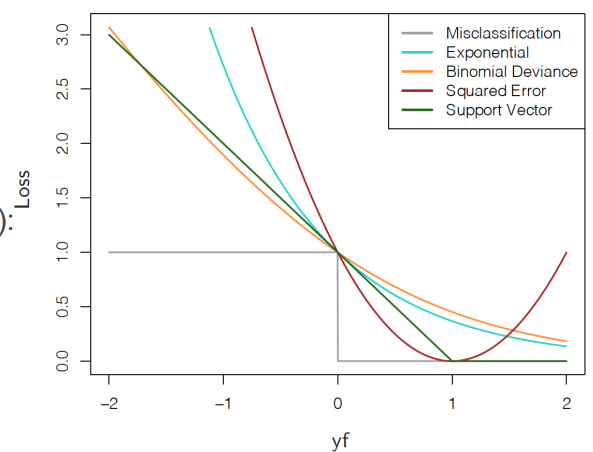
\includegraphics[scale=0.5]{assets/loss_functions.png}

  \begin{itemize}
    \item Misclassification 
    \[[\text{sign}(\hat{f}) \neq y]\]
    \item Exponential
    \[e^{-y\hat{f}}\]
    Punishes wrong predictions exponentially, so problematic when bayes error is high
    \item Cross entropy (Binomial deviance)
    \[\log(1+e^{-2y\hat{f}})\]
    Deals better with high Bayes error in the dataset
    \item Squared error
    \[(y-\hat{f})^2\]
    It does not decrease continuously, so unnecessary attention on correctly classified entities.
    \item Hinge loss (Support vector)
    \[\max(0,1-y\hat{f})\]
  \end{itemize}
\end{center}
\subsection{Comparing loss functions for regression}
\begin{center}
  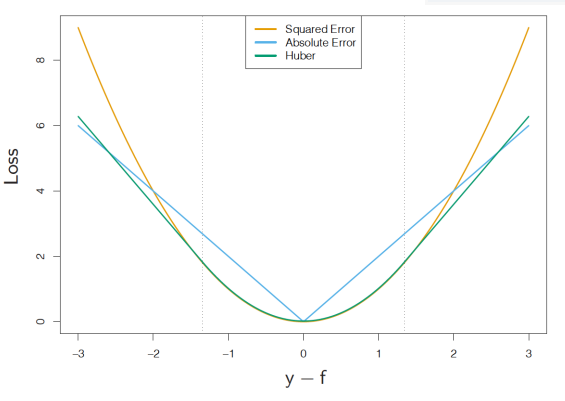
\includegraphics[scale=0.5]{assets/loss_functions_regression.png}

  \begin{itemize}
    \item Squared error
    \[(y-\hat{f})^2\]
    Less robust against outliers
    \item Absolute error
    \[|y-\hat{f}|\]
    \item Huber
    \[L\left(y,\hat{f}(x)\right) = \begin{cases}
      (y - \hat{f}(x))^2, & |y-\hat{f}(x)| < \delta \\
      2\delta|y-\hat{f}(x)| - \delta^2 & \text{otherwise}
    \end{cases}\]
  \end{itemize}
\end{center}

\subsection{Takeaway}
Some loss functions perform badly in certain situations
\section{Support Vector Machines}
\subsection{Perceptron Algorithm}
\subsubsection{Linear Separability}
As the name says, if you can partition the data with a 'line'

\begin{center}
  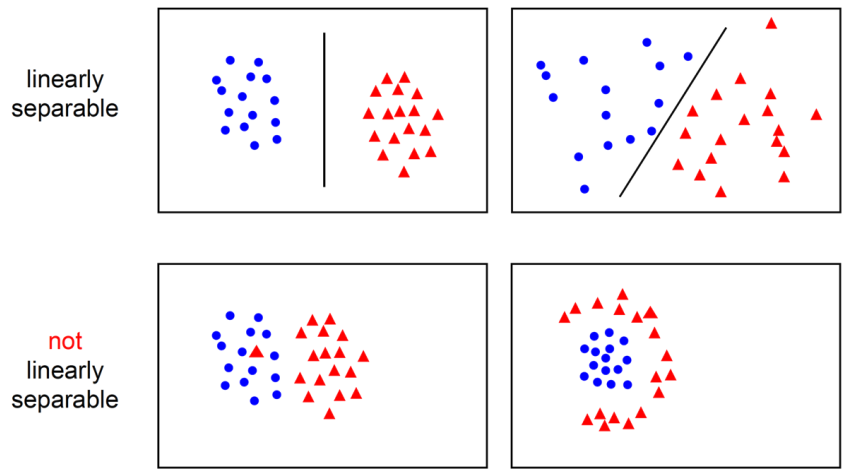
\includegraphics[scale=0.5]{assets/linear_separability.png}
\end{center}


A linear classifier has the form 
\[\hat{f}(x) = w^Tx + b\]
(basically the point-slope function but in multiple dimensions). $w$ is the normal to the line (weight vector), and $b$ is the bias

If we assume $x_i = (1,x_{i,1},\dots,x_{i,d})^T$ (as in linear regression) we can also leave the $b$ away
\[\hat{f}(x) = w^Tx\]

Also note that in 2D the discriminant is a line, in 3D it is a plane, etc..

\subsubsection{The perceptron classifier}
Given the training data $\{(x_i,y_i)\}$ with $x_i \in \mathbb{R}^d$ and $y_i \in \{-1,1\}$

How to find a weight vector $w$ so that the separating hyperplane correctly separates the two categories?
\begin{enumerate}
  \item Initialize $w = \mathbf{0}$
  \item While there is an $i$ such that $\hat{f}(x_i) y_i < 0$ do
  \[w := w - \alpha x_i \text{sign}\left(\hat{f}(x_i)\right)\]
\end{enumerate}
With $\alpha > 0$ being a learning rate

At convergence
\[w = \sum_{i=1}^N\alpha_ix_i\]
With $\alpha_i$ being the accumulated weight for training sample $x_i$

\begin{center}
  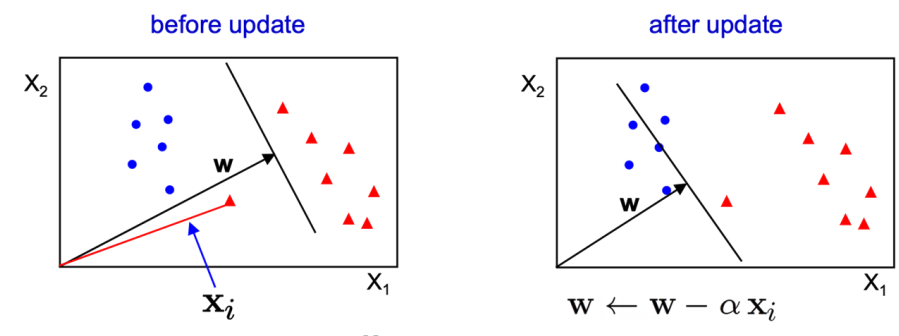
\includegraphics[scale=0.5]{assets/perceptron_algorithm_2d.png}
\end{center}
Convergence can be slow, but if there is a solution, the algorithm will find it. Separating line is also usually very close to training data
\subsection{Support Vectors}
What is the best $w$?

The idea is that we want the maximum margin solution, so that it is the most stable under perturbations.

\begin{center}
  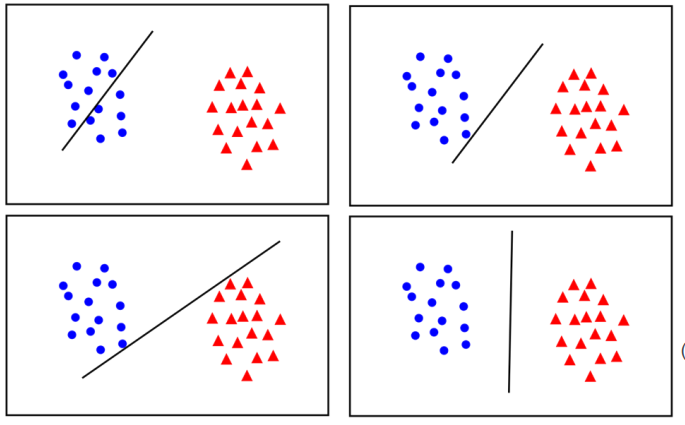
\includegraphics[scale=0.5]{assets/support_vector.png}

  We want bottom right
\end{center}
The support vectors are the values that are closest to the decision boundary. We want to equalize/maximize the distance from decision vectors to decision boundary.

\subsubsection{SVM Optimization Problem}
Distance $\delta(x_i,h)$ of data point $x_i$ to hyperplane $h$

\[\delta(x_i,h) = \frac{y_i\cdot (w^Tx_i + b)}{\|w\|}\]

In general, the length of vector $w$ does not matter, we usually fix $w$ so that the support vectors $x_j$ make $y_j(w^Tx_j + b) = 1$

The positive and negative support vectors have distance 
\[\delta(x_j,h) = \frac{1}{\|w\|}\]
We want to maximize this.

The standard formulation is instead, we want to minimize $\frac{\|w\|}{2}$


\[\max_w \frac{2}{\|w\|}\]
but subject to
\[y_i(w^Tx_i + b) \geq 1 \quad \text{for } \, i=1,\dots,N\]

Or Equivalently
\[\min_w \|w\|^2\] subject to the same constraints

This is a \textbf{quadratic optimization problem}

\subsection{Soft margin and Hinge Loss}
\begin{center}
  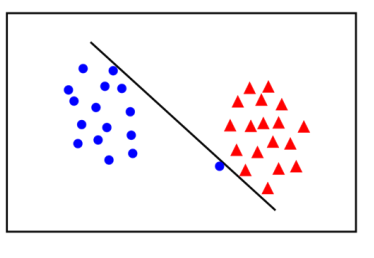
\includegraphics[scale=0.5]{assets/linear_separability_v2.png}

  A single outlier completely destroys the optimization problem. Possible, the large margin solution is better, even though one constraint is violated.
\end{center}
There is a trade-off between margin and number of mistakes


\subsubsection{Introducing 'slack' variables}
$\xi_i \geq 0$

The idea is that
\begin{itemize}
  \item $0 < \xi \leq 1$, the point is between margin and correct side of hyperplane. \textbf{Margin violation}
  \item $\xi > 1$. The point is \textbf{misclassified}
\end{itemize}

\begin{center}
  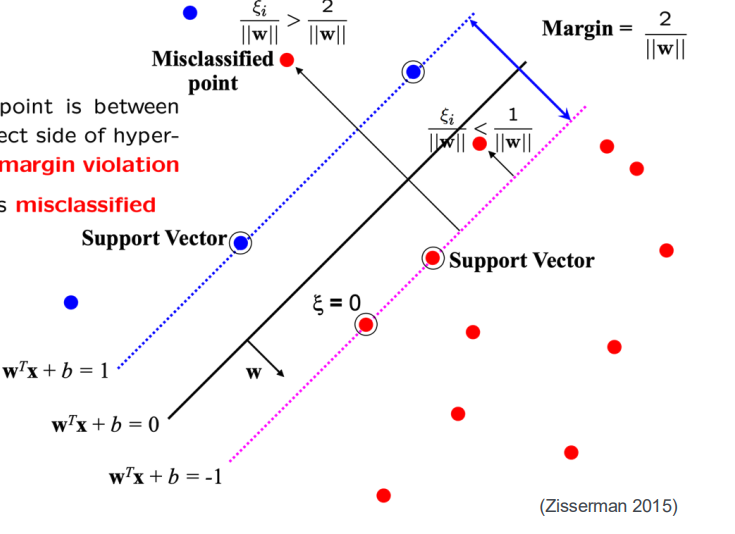
\includegraphics[scale=0.5]{assets/slack_variable.png}

  Note the formulas for the margins, we want to maximize those margins
\end{center}

\subsubsection{Soft margin solution}
\[\min_{w\in \mathbb{R}^d, \xi_i \in \mathbb{R}^+}\|w\|^2 + C\sum_{i=1}^N\xi_i\]
subject to
\[y_i(w^Tx_i + b) \geq 1 - \xi_i \quad \text{for } \, i=1,\dots,N\]

\begin{itemize}
  \item Every constraint can be satisfied if our $\xi_i$ is large enough.
  \item C is a \textbf{regularization parameter}. Small C allows constraints to be easily ignored (large margin), large C makes constraints hard to ignore (small margin), $C= \infty$ enforces all constraints
  \item Still quadratic optimization, but with a unique minimum.
  \item One hyperparameter C
\end{itemize}

\subsubsection{Loss function}
Given constraints
\[\xi_i \geq 0\]
\[y_i(w^Tx_i + b) \geq 1 - \xi_i\]

And we can rewrite $\xi_i$ as :
\[\xi_i = \max(0,1-y_i\hat{f}(x_i))\]

So we can optimize the unconstrained optimization problem over $w$
\[\min_{w\in\mathbb{R}^d} \underbrace{\frac{1}{C}\|w\|^2}_{\text{regularization}} + \sum_{i=1}^N \underbrace{\max(0,1-y_i\hat{f}(x_i))}_{\text{loss function}}\]


The points can be in three categories
\begin{enumerate}
  \item $y_i\hat{f}(x_i) > 1$. Outside margin. No loss
  \item $y_i\hat{f}(x_i) = 1$ On margin, no contribution to loss
  \item $y_i \hat{f}(x_i) < 1$ Violates margin constraint, contributes to loss
\end{enumerate}

SVM (Support Vector Machine) uses \textbf{Hinge loss} $\max(0,1-y\hat{f}(x_i))$


\subsection{Gradient Descent over convex function}
The idea is given a convex function, we want to climb 'down' the function, so go in the direction where

\[\frac{df(x)}{dx} = \nabla_xf(x)\]
is minimal


\subsubsection{Optimization}
Does this cost function have a unique solution?
\[\min_{w\in\mathbb{R}^d}C\sum_{i=1}^N\max(0,1-y_i\hat{f}(x_i))+ \|w\|^2\]
\begin{center}
  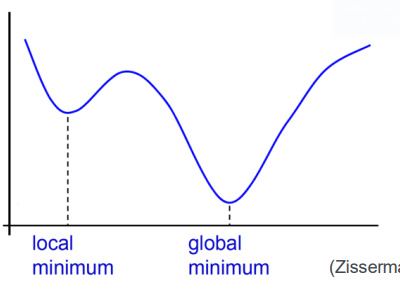
\includegraphics[scale=0.5]{assets/gradient_descent.png}
\end{center}

Can we find the solution through gradient descent?
\subsubsection{Convex functions}
A convex function $f:D\to\mathbb{R}$ is one that satisfies for any $x_0$, $x_1$ in D
\[f((1-\alpha)x_0 + \alpha x_1) \leq (1-\alpha) f(x_0) + \alpha f(x_1)\] 
\begin{center}
  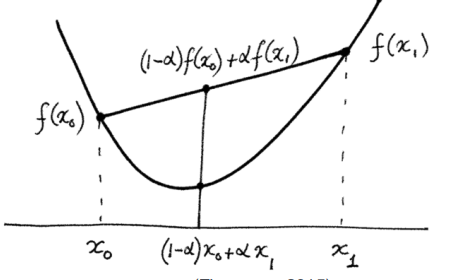
\includegraphics[scale=0.5]{assets/convex_functions.png}
\end{center}
A non-negative sum of convex functions is convex


We can prove that the hinge loss and regularization (SVM) is a convex function.

\subsubsection{Gradient Descent algorithm for SVM}
To minimize a cost function $C(w)$ use the iterative update

\[w_{t+1} := w_t - \eta_t \nabla_w C(w_t)\]
where $\eta$ is the learning rate

Let's rewrite the optimization problem as an average with $\lambda = \frac{2}{C}$
\[C(w) = \frac{1}{NC}\|w\|^2+ \frac{1}{N}\sum_{i=1}^N \max(0,1-y_i\hat{f}(x_i)) = \]
\[\frac{1}{N}\sum_{i=1}^N\left(\frac{\lambda}{2}\|w\|^2 + \max(0,1-y_i\hat{f}(x_i))\right)\]

and $\hat{f}(x_i) = w^T x + b$


\paragraph{Sub-gradient for Hinge loss}: 
\[L(x_i; y_i; w) = \max(0,1-y_i\hat{f}(x_i)), \hat{f}(x_i) = w^Tx_i + b\]

\begin{center}
  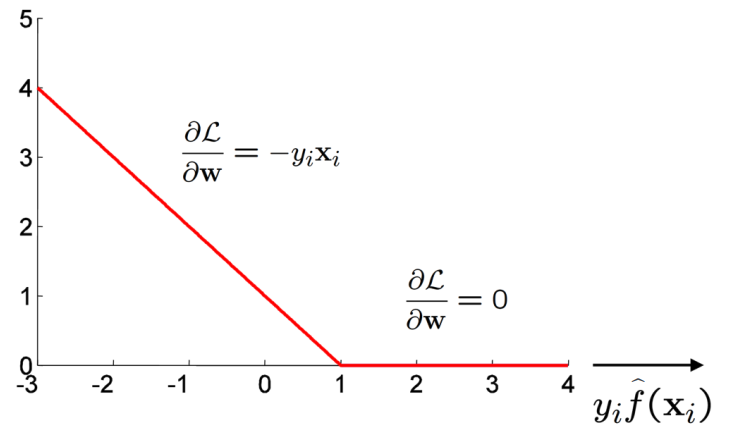
\includegraphics[scale=0.5]{assets/sub_gradient_hinge_loss.png}
\end{center}

\paragraph{Sub-gradient descent algorithm for SVM}: 
\[C(w) = \frac{1}{N}\sum_{i=1}^N\left(\frac{\lambda}{2}\|w\|^2 + \mathcal{L}(x_i,y_i;w)\right)\]
The iterative update is
\[w_{t+1} := w_t - \eta\nabla_wC(w_t) :=\]
\[:= w_t - \eta\frac{1}{N}\sum_{i=1}^N(\lambda w_t + \nabla_w\mathcal{L}(x_i,y_i;w))\]

So then, each iteration $t$ involves cycling through the training data with the updates
\[w_{t+1} := \begin{cases}
  w_t - \eta(\lambda w_t - y_ix_i) & \text{if }y_i\hat{f}(x_i) < 1 \\
  w_t - \eta\lambda w_t & \text{otherwise} 
\end{cases}\]

Note: The typical learning rate is $\eta_t = \frac{1}{\lambda t}$
\subsection{The dual problem}
\subsubsection{Primal vs dual problem}
SVM is a linear classifier $\hat{f}(x) = w^Tx +  b$

\textbf{The primal problem}: an optimization problem over $w$
\[\min_{w\in\mathbb{R}^d}\frac{1}{C}\|w\|^2 + \sum_{i=1}^N\max(0,1-y_i\hat{f}(x_i))\]

\textbf{The dual Problem}: Getting rid of the $w$ for a slightly different representation of $\hat{f}(x)$ that leads to the following representation
\[\hat{f}(x) = \sum_{i=1}^N \alpha_i y_i(x_i^Tx) + b\]
and a new optimization problem with the same solution, but several advantages


\subsubsection{Revisit optimization problem for hard margin case}

Minimize the quadratic form
\[\frac{\|w\|^2}{2} = \frac{w^T w}{2}\]
with constraint
\[y_i (w^Tx_i + b) \geq 1 \quad \forall i\]

The constraints will reach a value of 1 for at least one instance. If we include hard constraints into the loss function

\[\mathcal{L}(w,b,\alpha) = \frac{\|w\|^2}{2} - \sum_{i=1}^N\alpha_i(y_i(w^Tx_i + b) - 1)\]
failed constraints punish the objective function

\paragraph{Lagrange multiplier (mental excursion)}: We want to maximize function $f(x)$ under constraints $g(x) = a$. We can optimize with Lagrange multiplier $f(x) - \lambda(g(x) -a)$ instead

\paragraph{Algorithm for optimization with Lagrange Multiplier}

\begin{enumerate}
  \item Write down the Lagrangian $f(x) - \lambda (g(x) -a )$
  \item Take derivative w.r.t x, set to 0. Find estimate of $x$ that depends on $\lambda$
  \item Plug estimate into Lagrangian, take derivative w.r.t $\lambda$, set to zero and find optimal value for lagrange multiplier $\lambda$
  \item Plug in the lagrange multiplier in your estimate for $x$
\end{enumerate}

And if we remember from above
\[\mathcal{L}(w,b,\alpha) = \frac{\|w\|^2}{2} - \sum_{i=1}^N\alpha_i(y_i(w^Tx_i + b) - 1)\]

$\alpha_i$ are the Lagrange multipliers


\paragraph{Lagrangian primal problem}
\[\min_{w,b}\max_{\alpha} \mathcal{L}(w,b,\alpha)\]
under constraint $\forall i: \alpha_i \geq 0$

\paragraph{Finding the optimum}: Loss is a function of $w,b,\alpha$

We find the optimum using derivatives

\[\frac{\partial}{\partial b}\mathcal{L}(w,b,\alpha) = 0 \Rightarrow 0 = \sum_{i=1}^N\alpha_i y_i\]

\[\frac{\partial}{\partial w_j} \mathcal{L}(w,b,\alpha) = 0 \Rightarrow w_j = \sum_{i=1}^N\alpha_iy_ix_{i,j} \Rightarrow w = \sum_{i=1}^N \alpha_iy_ix_i\]

Substitution (not done by hand)
\begin{center}
  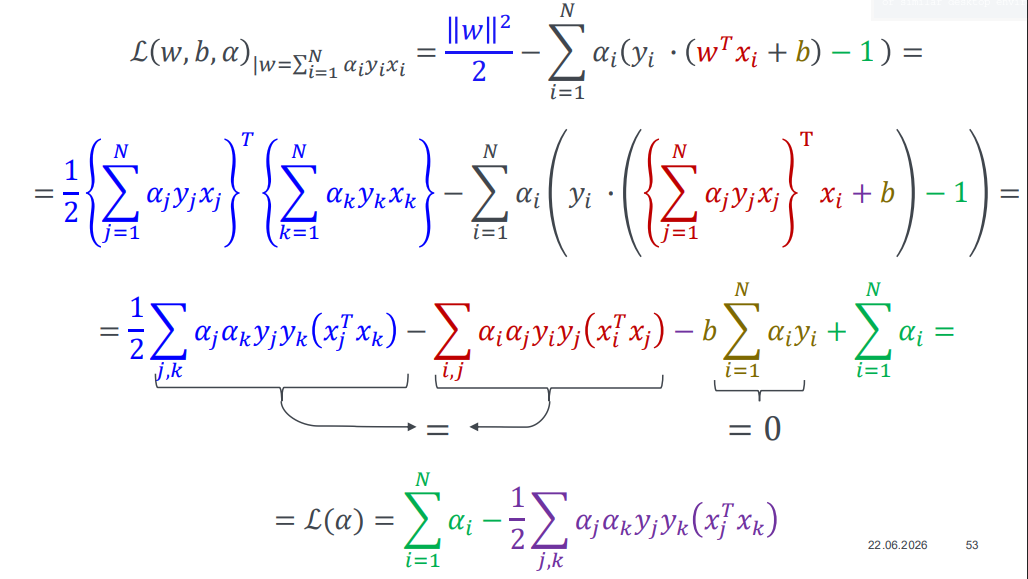
\includegraphics[scale=0.5]{assets/loss_substitution_gradient_descent.png}
\end{center}
\subsubsection{Wolfe-dual Problem}
\[\max_\alpha \sum_{i=1}^N \alpha_i - \frac{1}{2}\sum_{j,k} \alpha_j\alpha_ky_jy_k(x^T_jx_k)\]
subject to $\forall i: \alpha_i \geq 0$ and $0 = \sum_{i=1}^N\alpha_iy_i$

This problem is solvable with quadratic programming. It gives us the classification function
\[\hat{f}(x) = \sum_{i=1}^N\alpha_i \cdot y_i \cdot x_i^T x + b\]
\subsubsection{Summary: Primal and dual formulations}
Primal version of the classifier
\[\hat{f}(x) = w^Tx + b\]

Dual version of the classifier
\[\hat{f}(x) = \sum_{i=1}^N \alpha_i y_i x_i^T x + b\]
The dual form seems to work like a kNN classifier, because it requires training points $x_i$, but in practice many of the $\alpha_i$ are zero. The ones that are non-zero define the support vectors $x_i$



The Lagrangian primal problem
\[\min_{w,b}\max_\alpha \mathcal{L}(w,b,\alpha)\]
subject to $\forall i: \alpha_i \geq 0$

The Lagrangian dual problem
\[\max_\alpha\sum_{i=1}^N\alpha_i - \frac{1}{2}\sum_{j,k}\alpha_j\alpha_ky_jy_k(x_j^Tx_k)\]
Subject to $\forall i: \alpha_i \geq 0 $ and $0 = \sum_{i=1}^N\alpha_iy_i$

\subsection{Kernelization Tricks in SVMs}

The thing is that not all classes can be separated via a hyperplane. The solution is \textbf{feature engineering}

\subsubsection{Feature engineering using $\phi(x)$}
Classifier: Given $x_i \in \mathbb{R}^d, \phi: \mathbb{R}^d \to \mathbb{R}^D$, $w\in\mathbb{R}^D$

\[\hat{f}(x) = w^T\phi(x) + b\]

Learning
\[\min_{w\in\mathbb{R}^D}\frac{1}{C}\|w\|^2 + \sum_{i=1}^N \max(0,1-y_i\hat{f}(x_i))\]
\begin{center}
  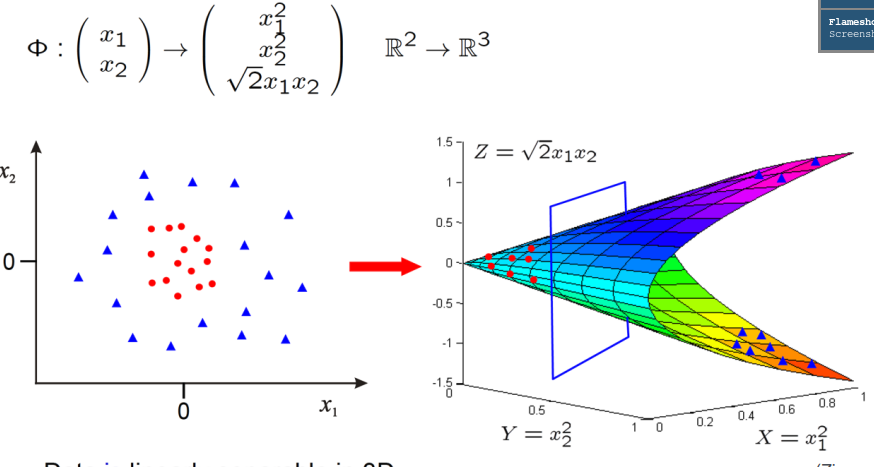
\includegraphics[scale=0.5]{assets/feature_engineering.png}

  The effect of applying functions when feature engineering, allows us to generate a valid hyperplane.
\end{center}

The idea is usually mapping to a higher dimensional space $D$ where the data can be separated with a hyperplane.

However, if $D \gg d$ there are many more parameters to learn for $w$

\subsubsection{Dual classifier in transformed feature space}
Classifier
\[\hat{f}(x) = \sum_{i=1}^N \alpha_i y_i x_i^Tx + b \Rightarrow\]
\[ \Rightarrow \hat{f}(x) = \sum_{i=1}^N \alpha_i y_i \phi(x_i)^T\phi(x) + b \]

And for learning its analogous
\[\max_\alpha\sum_{i=1}^N\alpha_i - \frac{1}{2}\sum_{j,k}\alpha_j\alpha_ky_jy_k(\phi(x_j)^T\phi(x_k))\]
Subject to the usual.


\paragraph{Kernels}
\[k(x_j,x_k) = \phi(x_j)^T \phi(x_k)\]

\subsubsection{Dual classifier using kernels}
The same as above only with the kernel substitution

Classifier
\[\hat{f}(x) = \sum_{i=1}^N \alpha_i y_i k(x_i, x) + b \]


Learning
\[\max_\alpha\sum_{i=1}^N\alpha_i - \frac{1}{2}\sum_{j,k}\alpha_j\alpha_ky_jy_kk(x_j,x_k)\]

\subsection{Kernels}
Formal definition: Given mapping $\phi: \mathcal{X} \to \mathcal{H}$ from input space $\mathcal{X}$ to a possibly infinitely-dimensional space $\mathcal{H}$. A kernel function $k$ is defined as 
\[k(x,x') = \langle \phi(x), \phi(x')\rangle_{\mathcal{H}}\]

It computes the inner product between the images of x and x', but without needing to know $\phi$ explicitly.

\subsubsection{Properties}
\begin{itemize}
  \item Symmetric
  \item Positive semi-definite.
\end{itemize}

\subsubsection{Examples}
\begin{itemize}
  \item Linear kernels:
  \[k(x,x') = x^Tx'\]
  \item Polynomial kernels:
  \[k(x,x') = (1+x^Tx')^d\]
  \item Gaussian kernels:
  \[k(x,x') = e^{-\frac{\|x-x'\|^2}{2\sigma^2}} \quad \sigma > 0\]
  Infinite dimensional feature space. Also called Radial basis function kernel (RBF)
\end{itemize}

\subsection{Transductive Classification}
They are special SVM's that use test data, not only training data with the Objective function

$$\min_{w, b, \xi, \xi^*} \frac{1}{2} \Vert{}w\Vert{}^2 + C \sum_{i=1}^{m} \xi_i + C^* \sum_{j=1}^{k} \xi_j^*$$
\begin{itemize}
  \item $\frac{1}{2}\Vert{}w\Vert{}^2$: Standard SVM objective to maximize the margin ($\frac{2}{\Vert{}w\Vert{}}$).
  \item $C \sum_{i=1}^{m} \xi_i$: Penalty for misclassifications or margin violations on the labeled training data ($m$ samples).
  \item $C^* \sum_{j=1}^{k} \xi_j^*$: Penalty for margin violations on the unlabeled test data ($k$ samples).
  \item $C$ and $C^*$: Hyperparameters balancing the trade-off between margin width, training error, and test set assignment confidence.
\end{itemize}
Subject to
$$y_i (w^T x_i + b) \ge 1 - \xi_i \quad \forall i = 1, \dots, m$$
$$y_j^* (w^T x_j^* + b) \ge 1 - \xi_j^* \quad \forall j = 1, \dots, k$$
$$\xi_i \ge 0, \quad \xi_j^* \ge 0$$
\section{Neural Networks}
\subsection{Biological vs Artificial}
The workings on natural neural networks motivated research on artificial neural networks.
\subsection{Reminder: Logistic Regression}
Logistic regression is a machine learning method where you predict probabilities of an event ocurring. Mainly used for binary classification tasks.

You have a \textbf{model}, composed of
\begin{itemize}
  \item A linear function $z = x^T\beta$
  \item A non-linear activation function
  \[y = \frac{e^z}{1+e^z}\]
  \item Together they form
  \[\hat{f}(x) = \frac{e^{x^T\beta}}{1+e^{x^T\beta}}\]

  \begin{center}
    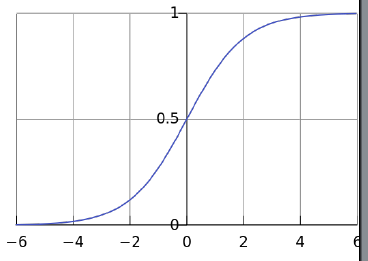
\includegraphics[scale=0.5]{assets/logistic_regression.png}
  \end{center}
\end{itemize}
And you also have a loss function, based on \textbf{cross entropy} and \textbf{regularization}
\[\text{loss}^{\text{logistic}}(\beta) = \sum_{i=1}^NH(\overline{y}_i , P(\cdot | X = x_i)) + \lambda ||\beta||^2\]
Note: (the $\lambda ||\beta^2||$ is the L2 Regularization that penalizes large weights)


To solve, you adapt the weights, based on something like \textbf{gradient descent}

\subsubsection{Logistic regression for binary cases}
In a two class example, you want yo predict conditional probabilities. (Two class example)
\[P(G = 1 | X = x) = \frac{e^{x^T \beta}}{1+e^{x^T\beta}}\]
\[P(G = 2 | X = x) = \frac{1}{1+e^{x^T\beta}}\]


\begin{center}
  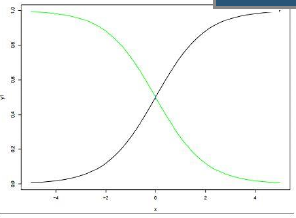
\includegraphics[scale=0.5]{assets/logistic_regression_binary.png}
\end{center}

\paragraph{Problem: Learning XOR with logistic regression}: So XOR is a diagonal problem, so it cannot be cleanly divided with a single linear classifier (which the logistic regression is).
\begin{center}
  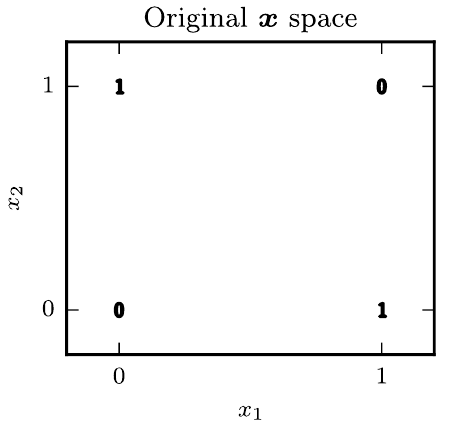
\includegraphics[scale=0.5]{assets/xor_problem.png}
\end{center}

This is because logistic regression can only draw a hyperplane (a line in 2D, and a plane in 3D), so it cannot inherently learn the XOR problem.

To fix this, there are two main methods
\begin{itemize}
  \item Kernelization: Modifying the data so that it is separable
  \item Composition of non-linear functions (which is the basis of Neural Networks)
\end{itemize}
\subsection{Feed-Forward Networks and Activation Functions}
\subsubsection{Network: Composing Functions}
A three layer network
\[f(x) = f^{(3)}(f^{(2)}(f^{(1)}(x)))\]
With the last layer $f^{(3)} = \hat{y}$ being the output layer.

\paragraph{Composition of linear functions for XOR Problem? }
If we have layer 1 (hidden layer)
\[h = f_1(x) = W^T x + c\]
And layer 2 (output layer)
\[y = f_2(h) = w^T h + b\]

Then $f(x) = w^TW^T x$, and the result is still linear. So combinations of linear functions still yields linear functions, so we cannot use it for the XOR problem.
\subsubsection{One Layer in a Feed-Forward Network}
The output of a single unit (neuron) within an arbitrary layer $i$ is defined by a linear combination of non-linear features:
\[f^{(i)}(x) = w_{i,0} + \sum_{j=1}^{l_i} w_{i,j} \cdot \phi(x; \theta_i) = \phi(x;\theta_i)^T w_i\]

With:
\begin{itemize}
  \item $l_i$ being the number of incoming features (the width/dimension of the preceding layer).
  \item $w_{i,j}$ being the weight in layer $i$ associated with the $j$-th incoming feature, and $w_{i,0}$ being the bias term.
  \item $\phi(x;\theta_i)$ being a basis function used to extract features. Instead of hand-crafting this function, deep learning makes it learnable by nesting a parameterized linear component inside a fixed, non-linear activation function $g(z)$:
  \[\phi(x;\theta_i) = g(x^T\theta_i)\]
  where $\theta_i$ represents the weights of the previous layer that generate these features.
\end{itemize}
\paragraph{Activation functions}: This has been a long debate on which to use, below are the most common
\begin{itemize}
  \item Sigmoid: $g(z) = \sigma(z) = \frac{e^z}{1 + e^z}$
  \item ReLU: $g(z) = \max\{0,z\}$
  \item Leaky ReLU: $g_\alpha(z) = \max\{\alpha z, z\}$
  \item Maxout unit: $g(z) = \max_j\{z_j\}$
  \item Absolute value: $g(z) = |z|$
  \item Hyperbolic tangent: $g(z) = \tanh(z)$
  \item Radial Basis function: $g(z) = e^{-\frac{1}{2}||z_j - c_j||^2}$
\end{itemize}
The most used is ReLU because of speed and simplicity, but it lacks differentiability at 0.

Using this method, we CAN solve the XOR problem

\subsubsection{Universal Approximation Theorem}
Let $\varphi: \mathbb{R}\to\mathbb{R}$ be a nonconstant, bounded, and monotonically-increasing continuous function.

Then let $\mathcal{C}$ denote the space of continuous functions  on $[0,1]^m$

Given \textbf{any} $\varepsilon > 0$ and \textbf{any} function $f \in \mathcal{C}$

there exist, $N \in \mathbb{N}$, $v_i,b_i \in \mathbb{R}$, $w_i \in \mathbb{R}^m$, with $i=1,...,N$ where
\[F(x) := \sum_{i=1}^N v_i \varphi(w_i^Tx + b_i)\]
and 
\[|F(x)-f(x)| < \varepsilon \quad \forall x \in [0,1]^m\]
So translated, on compact spaces, sufficiently broad neural networks can approximate any continuous function arbitrarily well. However, this is not practical, as there is no guarantee that N is even non-exponential.

As a summary, we are still missing a Loss function and the solving for One-Layer Feed Forward Networks.

\subsection{Backpropagation}
It is used to compute the Loss $L(\theta)$ considering data $y$ and $\hat{y}$ (output prediction)


\subsubsection{Computation Graphs: Language for representing the backpropagation problem}
It's a language to represent mathematical expressions using graphs. They are pretty self explanatory.

\begin{center}
  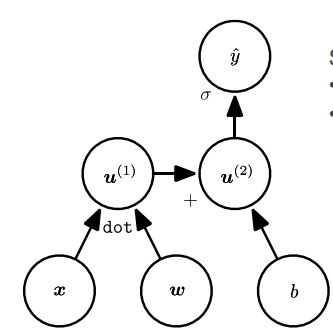
\includegraphics[scale=0.5]{assets/computational_graphs.png}
\end{center}
\paragraph{Notational Conventions}
There are $n$ many nodes in the graph, topologically sorted. $u_1,...,u_n$

The input layers with values for $k$ nodes are $u_1,...,u_k$.

The set of values of parent of node $i$ is $\mathbb{A}^{(i)}$

Operator for node $i$ is $f^{(i)}$

Output layer with $l$ nodes $u_{n-l+1},...,u_n$

So in the above example the distribution would be


\begin{itemize}
  \item $u_1 = x_1$
  \item $u_2 = w$
  \item $u_3 = b$
  \item $u_4 = u^{(1)}$
  \item $u_5 = u^{(2)}$
  \item $\mathbb{A}^{(4)} = \{u_1, u_2\} = \{x, w\}$
  \item $\mathbb{A}^{(5)} = \{u_3, u_4\} = \{b, u^{(1)}\}$
  \item $\mathbb{A}^{(6)} = \{u_5\}$
  \item $f^{(4)} = dot$
  \item $f^{(5)} = +$
  \item $f^{(6)} = \sigma$
  \item $u_{6} = \hat{y}$ 
\end{itemize}

\paragraph{Forward propagation in computational graph}: 
\begin{algorithm}
for i = k+1,...,n do: \\
$\quad \mathbb{A}^{(i)} \leftarrow \{u_j | j \in parent(u_i)\}$ \\
$\quad u_i \leftarrow f^{(i)}(\mathbb{A}^{(i)})$\\
end for\\
return $u_n$\\
\end{algorithm}

\subsubsection{Backpropagation}
Below is an easy example
\begin{center}
  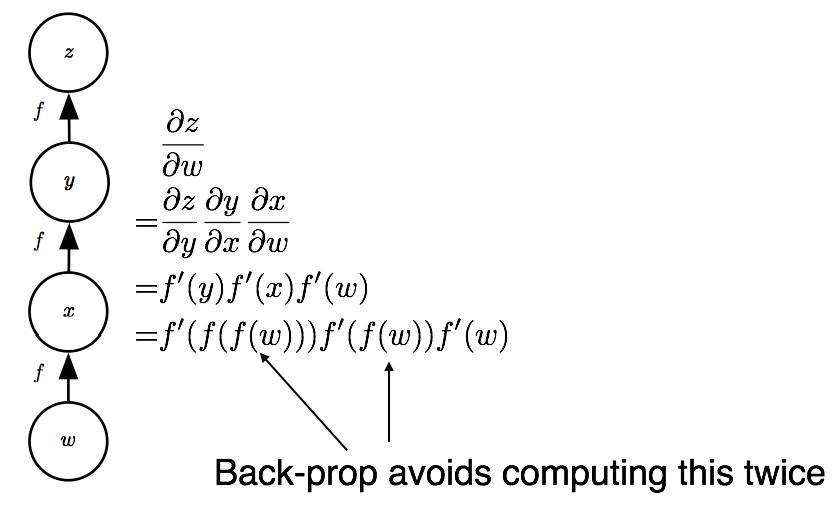
\includegraphics[scale=0.5]{assets/backpropagation.png}
\end{center}

\paragraph{Example in a tiny computational graph}: 
\begin{center}
  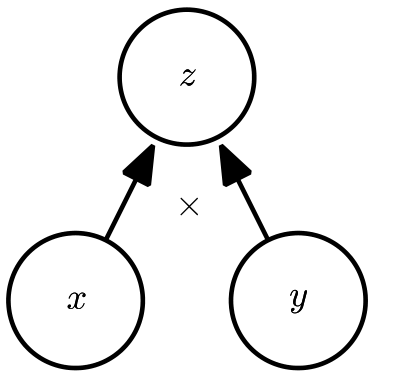
\includegraphics[scale=0.5]{assets/backpropagation_2.png}
\end{center}
Imagine we have input $x=1$, $y=2$ and target $z=3$. The forward result is $\hat{z} = x\cdot y = 2$

If we assume MSE as our loss function
\[J = L(\hat{z},z) = \frac{1}{2}(\hat{z}-z)^2 = \frac{1}{2}\]

We want to now compute the effect of $\hat{z}$ on the loss function. (We use here partial and not gradient because $\hat{z}$ is a scalar and not a vector)
\[\frac{\partial J }{\partial \hat{z}} = \frac{\partial}{\partial \hat{z}}\left[\frac{1}{2}(\hat{z} - z)^2\right] = (\hat{z} - z)\]
When plugging in our numbers we get
\[\frac{\partial J}{\partial \hat{z}} = (2-3) = -1\]
This means the gradient direction is negative. Now via the chain rule we can get the effect of $x$ and $y$
\[\nabla_{(x,y)}J = \begin{pmatrix}
  \frac{\partial J}{\partial x} \\
  \frac{\partial J}{\partial y} 
\end{pmatrix} = \begin{pmatrix}
  \frac{\partial J}{\partial \hat{z}}\frac{\partial \hat{z}}{\partial x} \\
  \frac{\partial J}{\partial \hat{z}}\frac{\partial \hat{z}}{\partial y}
\end{pmatrix} = \begin{pmatrix}
  -2 \\
  -1
\end{pmatrix}\]

Since derivative measures change, a negative gradient means that increasing $x$ or $y$ will decrease the loss $J$.


So for example for $y$
\[y^{new} = y - \eta \nabla_y = y - \eta(-1)\]
With learning rate $\nabla$


\subsection{Modelling a Feed-Forward Network predicting a Bernoulli distribution}
Note: A Bernoulli distribution only has two outcomes: $1$ with probability $p$ and $0$ with probability $1-p$.

\subsubsection{Loss function with Maximum Likelihood}
Given training data $\{(x_i,y_i)\}_{i=1}^N$ where $x_i \in \mathbb{R}^d$ and $y_i \in \{0,1\}$.

The cross-entropy loss over the dataset is defined as:
\[L(\theta) = \mathbb{E}_{\text{data}}(-\log P(y|x)) = - \frac{1}{N}\sum_{i=1}^N \log P(y_i|x_i)\]
\subsubsection{Probabilistic Model and Activation}
Let the linear logit layer be defined as $z = w^T x + b$. Intuitively, we want $z$ to be a large positive number when the true label $y=1$, and a large negative number when $y=0$. This relationship is compactly expressed by modeling the unnormalized conditional log-probability as:
\[\log P(y|x) \propto (2y-1)z \Rightarrow P(y \mid x) \propto e^{(2y-1)z}\]
Note that these scores are unnormalized (meaning they don't sum up to one). This is fixed below

To handle both the $y=1$ and $y=0$ cases simultaneously with a single elegant expression, we map the binary target $y \in \{0,1\}$ to the sign domain $y' = 2y - 1 \in \{-1, 1\}$:
\begin{itemize}
    \item If $y = 1 \implies y' = 1$ (demanding a large positive $z$)
    \item If $y = 0 \implies y' = -1$ (demanding a large negative $z$)
\end{itemize}

Normalizing these exponential probabilities (by dividing with all the possible outputs) so that $P(y=1|x) + P(y=0|x) = 1$ yields:
\[P(y|x) = \frac{e^{yz}}{\sum_{y'=0}^1 e^{y'z}} = \frac{e^{(2y-1)z}}{1 + e^{(2y-1)z}} = \sigma((2y-1)z)\]
where $\sigma(a) = \frac{1}{1+e^{-a}}$ is the standard sigmoid activation function.
\subsubsection{Negative Log-Likelihood Formulation}
Taking the negative log of the normalized probability for a single sample gives:
\[L_i(\theta) = -\log P(y|x) = -\log \sigma((2y-1)z)\]

Using the identity $-\log \sigma(a) = \zeta(-a)$, where $\zeta(a) = \log(1 + e^a)$ is the softplus function, the loss simplifies cleanly to:
\[L_i(\theta) = \zeta((1-2y)z)\]
\subsubsection{Softplus function $\zeta$}
\[\zeta(x) = \log(1+e^x)\]
\[\frac{d\zeta}{dx}(x) = \sigma(x)\]
\[\log(\sigma(x)) = -\zeta(-x)\]

\subsubsection{Summary: Learning Bernoulli Output}
The model is $\hat{f}(x) = \sigma(w^T x)$

The loss function is \textbf{softplus}
\[L(\theta) = \zeta((1-2y)z)\]

And we solve with gradient descent
\[\frac{d\zeta(x)}{dx} = \sigma(x)\]

\subsubsection{Softmax vs Softplus}
\begin{itemize}
  \item Softplus operates on a single scalar input to ensure the output is strictly positive ($>0$).
  \item Softmax operates on a vector of inputs to convert them into a normalized probability distribution ($\sum = 1$).
\end{itemize}
\subsection{Modelling a Feed-Forward Network predicting a Multinoulli distribution}
In Bernoulli it was
\[\hat{y} = P(y= 1|x)\]
With Multinoulli
\[\hat{y}_i = P(y=i | x)\]
With $\hat{y} = (\hat{y}_1,...,\hat{y}_n)$ being the vector of predicted values from our Neural Network for $n$ different classes. With the property of

\[\forall i \quad \hat{y}_i \in [0,1]\]
and
\[\sum_{i=1}^n \hat{y}_i = 1\]

Basically, a Bernoulli distribution with more than 2 outcomes, like rolling a 6-sided die.


So before, $z$ and $b$ were scalars and $w$ and $h$ were vectors, now $z$ and $b$ and $h$ (can also be called $x$, depends if its true input or previous layer) are vectors  and $w$ is a matrix.

We also use the \textbf{softmax function}
\[\text{softmax}(z)_i = \frac{e^{z_i}}{\sum_j e^{z_j}}\]

The issue is that the denominator can overflow when computing inside a computer. So we pick $c := \max_i z_i$ and just do
\[\text{softmax}(z)_i = \frac{e^{z_i - c}}{\sum_j e^{z_j-c}}\]
This is called \textbf{stable softmax}

\subsubsection{Multinoulli Loss Function (Cross-Entropy)}
For a single data record, let the true class label be represented as a one-hot encoded vector $y = [0, \dots, 0, 1_i, 0, \dots, 0]^T$ (often written simply as $y = i$, where $i$ is the correct class index). 

The cross-entropy loss measures the distance between the true data distribution and our model's learned distribution:
\begin{align*}
L_i(\theta) &= -\sum_{j} y_j \log(\text{softmax}(z)_j) \\
&= -\log(\text{softmax}(z)_i) \\
&= -\log \left( \frac{e^{z_i}}{\sum_j e^{z_j}} \right) \\
&= - \left( \log e^{z_i} - \log \sum_j e^{z_j} \right) \\
&= \log \sum_j e^{z_j} - z_i
\end{align*}

This final form shows that to minimize the loss, the network must pull the correct logit $z_i$ up, while pushing the sum of all exponentials $\sum_j e^{z_j}$ down.
\subsection{Modeling a Mixture Density distribution}
Imagine we want to model a distribution of dogs, two breeds: Chihuahuas and Siberian Huskys. They vary wildly in weight, so the final distribution will be a \textbf{mixture of gaussians}.

\begin{center}
  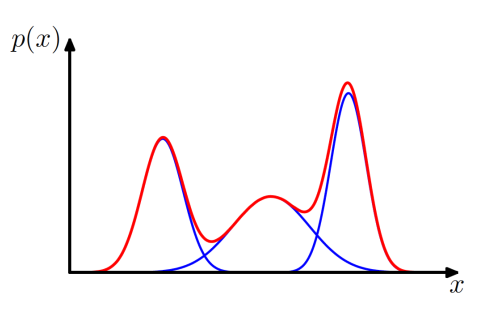
\includegraphics[scale=0.5]{assets/regression_gaussian_mixture.png}
  
  This is the regression result of regression of a Gaussian Mixture. Luckily this is univariate, for multivariate it turns even harder, with multiple dimensions.  
\end{center}

The approach mainly to solve this is to use a Multinoulli softmax layer to try to categorize the groups, and then computing the means, and then the covariance matrices

\begin{center}
  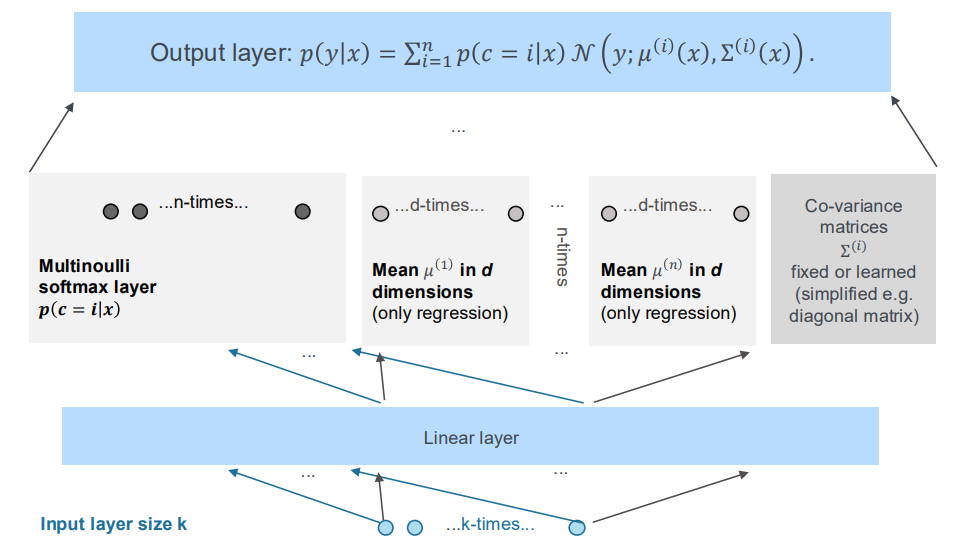
\includegraphics[scale=0.5]{assets/regression_gaussian_mixture_2.png}
\end{center}

The Loss function used is usually the \textbf{Mean Squared Error}, with some variations.


The prediction is then
\[\mathbb{E}[y|x] = \int y P(y|x) dy  = \sum_{i=1}^N P(c= i)\mu^{(i)}(x)\]

\subsection{Optimizing Gradient Descent}
\subsubsection{Initialization}
\begin{itemize}
  \item The initialization of weights is important, there are some heuristics
  \item Choose random weights that don't grow or vanish the gradients. Choose each weight vector $W_{l,i\cdot}$ to point in a uniform random direction.
  \item Choose biases $b_{l,i}$ randomly so that ReLU hinges over the input well
\end{itemize}
\subsubsection{Optimization}
\begin{itemize}
  \item For small data size: Compute the loss and it's gradient 
  \[\sum_{i=1}^n \nabla_\beta l(f_\beta(x_i), y_i)\]
  Then use classic gradient-based optimization methods
  \item For large data size the $\sum_{i=1}^N$ is largely inefficient! So we adapt weights based on much smaller data subsets, \textbf{mini batches}
\end{itemize}
\paragraph{Newton's method in optimization (1D)}: To minimize $f(x)$, iterate $t= 0,1...$ for $x_t$ to approach minimum

Taylor expansion
\[f(x_t + \varepsilon) \approx f(x_t) + f'(x_t)\varepsilon + \frac{1}{2}f''(x_t)\varepsilon^2\]

If we derive and set to zero
\[\varepsilon = -\frac{f'(x_t)}{f''(x_t)}\]

So then to optimize, we just set $x_{t+1} = x_t + \varepsilon$


And to do in several dimensions: We call the gradient 
\[g_f(x) = \nabla f(x) = \left(...,\frac{\partial f(x_1,...,x_i,...)}{\partial x_i},...\right)^T\]

The Hessian is then 
\[H_f(x) = \nabla^2 f(x) = \begin{pmatrix}
  ... & ... & ... \\
  ... & \frac{\partial^2 f(x_1,...,x_i,...)}{\partial x_i^2} & .... \\
  ... & ... & ... \\
\end{pmatrix}\]
So then $x_{t+1} = x_t - \eta [H_f(x_t)]^{-1}g_f(x_t)$

With $\eta < 1$ we dampen the search.

\paragraph{Illustrating and Computing the Hessian}: The Hessian is symmetric, and largest and smallest eigenvector illustrate the largest and smallest curvature.

\begin{center}
  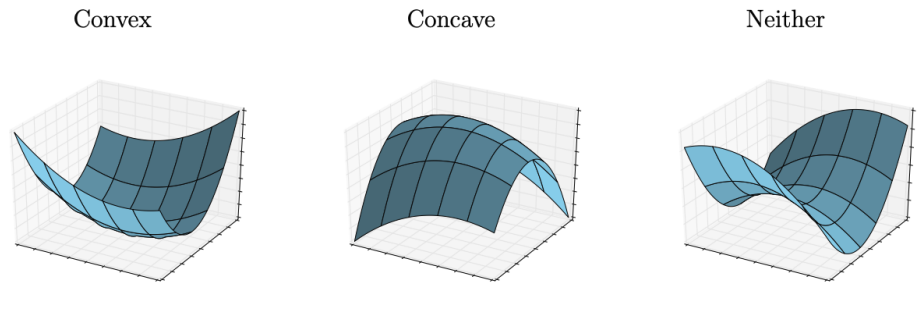
\includegraphics[scale=0.5]{assets/hessian.png}
\end{center}

To compute, inverting the Hessian is expensive and should be avoided. So we do not compute $h(x_t) = [H_f(x_t)]^{-1} g_f(x_t)$. Rather we solve the linear equation
\[H_f(x_t)h(x_t) = g_f(x_t)\]

\paragraph{Convergence}: For strongly convex functions with Lipschitz Hessian matrix, meaning
\[||\nabla ^2 f(x) - \nabla^2 f(y)||_{op} \leq L||x-y||_2\]
we have quadratic convergence.

Convexity is generally not given for neural networks, but for other ML methods (SVM).

\textbf{Summary: Convergence is not typically guaranteed for NN, but practically, the high dimensionality usually allows for avoiding many local minima}

\subsubsection{Stochastic Gradient Descent}
So we instead compute the loss and gradient for a mini-batch $\hat{D} \subset D$ of fixed size $k$
\[L(\beta, \hat{D}) = \sum_{i\in \hat{D}} l(f_\beta (x_i), y_i)\]
And the gradient
\[\nabla_\beta L(\beta,\hat{D}) = \sum_{i\in \hat{D}} \nabla_\beta l(f_\beta (x_i), y_i)\]
\paragraph{Naive Stochastic Gradient Descent}: We iterate
\[\beta \leftarrow \beta - \eta \nabla_\beta L(\beta,\hat{D})\]
The choice of $\eta$ is key for convergence. We can use exponential cooling $\eta = \eta_0^t$

\paragraph{Adding Momentum}: SGD with momentum
\[\Delta \beta \leftarrow \alpha \Delta \beta - \eta \nabla_\beta L(\beta,\hat{D})\]
\[\beta \leftarrow \beta + \Delta \beta\]

And with \textbf{Nesterov Accelerated Gradient (NAG)}
\[\Delta \beta \leftarrow \alpha \Delta \beta - \eta \nabla_\beta L(\beta + \Delta \beta,\hat{D})\]
\[\beta \leftarrow \beta + \Delta \beta\]

\subsection{ADAM - Adaptive Moment Estimation}
Will not appear in exam.
\subsection{Regularization in DNNs: Lasso, Ridge and Constraints}
Regularization is defined as any modification done to a learning algorithm intended to reduce its generalization error, but not its training error.

DNN = Deep Neural Network
\subsubsection{Paramer Norm Penalty}
Regularized loss function
\[\tilde{J}(\theta; X , y) = \underbrace{J(\theta; X,y)}_{\text{Unregularized}} + \alpha\underbrace{\Omega(\theta)}_{\text{Regularizer on parameters}}\]

Note: $w$ only denotes the weights, while $\theta$ refers to \textbf{all parameters}

\subsubsection{$L^2$ Parameter Regularization}
\[\tilde{J}(w; X , y) = J(w; X,y) + \frac{\alpha}{2}w^T w\]
The bias vectors are usually not regularized

So the regularized gradient
\[\nabla_w \tilde{J}(w; X, y) = \nabla_w J(w; X,y) + \alpha w\]

If we use the regularized gradient for the weight updating.
\[w \leftarrow w - \varepsilon(\alpha w + \nabla_wJ(w; X,y))\]
\subsubsection{$L_1$ and $L_2$ regularization by weight decay}
Add penalty for every weight (Ridge or Lasso), and in practice, $L_1$ makes the weights become sparser than $L_2$ ($L_1$ pushes the weights toward 0 more often)

\subsubsection{Column-Wise (Matrix) Regularization}
In multi-layer models or multi-output regression, the weights for layer $l$ form a 2D matrix $W_l \in \mathbb{R}^{n \times m}$:

\[
W_l = \begin{pmatrix}
  w_{l,1,1} & \dots & w_{l,1,m} \\
  \vdots & \ddots & \vdots \\
  w_{l,n,1} & \dots & w_{l,n,m}
\end{pmatrix}
\]

where $n$ is the number of output units, $m$ is the number of input units, and $w_{l,i,j}$ represents the weight connecting input $j$ to output $i$.

To apply $L_2$ regularization (Ridge) to a weight matrix, we use the \textbf{Frobenius norm} $\|W_l\|_F$, which sums the squared magnitude of every individual weight in the matrix:

\[
\|W_l\|_F^2 = \sum_{i=1}^n \sum_{j=1}^m |w_{l,i,j}|^2
\]

\subsubsection{Regularization in DNNs: Data Augmentation}

You can generate more data by taking the data you have and modifying it slightly. Rotate it, add some noise, flip it. You basically get more data for free. But be careful (a rotated 6 is a 9).

\paragraph{Label Smoothing: Injecting noise at output target}

Most datasets have some number of mistakes in the $y$ labels. It can be harmful to maximize $P(y|x)$ if $y$ is a mistake.

The solution can be model the noise at the label
\[\frac{\varepsilon}{k-1},...,1-\varepsilon,\frac{\varepsilon}{k-1},...\]

\paragraph{Injecting noise into the weights}: We can wiggle all the weights with some noise $\varepsilon_W$

We propagate with wiggle weights to compute $\hat{y}_{\varepsilon_W}$

This aims to avoid getting stuck at local minima
\subsubsection{Multi-task learning}
From one data point $x$ several outputs $y^{(i)}$ representing different tasks

\subsubsection{Early stopping}
\begin{center}
  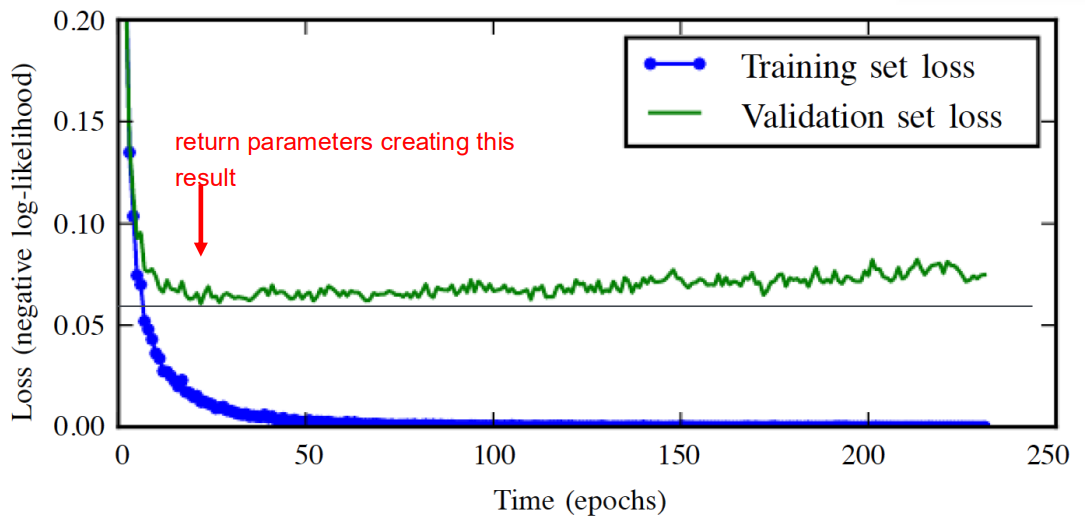
\includegraphics[scale=0.5]{assets/early_stopping.png}

  As you can see, to many epochs lead to overfitting, we want to return the optimal result for the validation set loss
\end{center}

\subsubsection{Adversarial Examples}
\begin{center}
  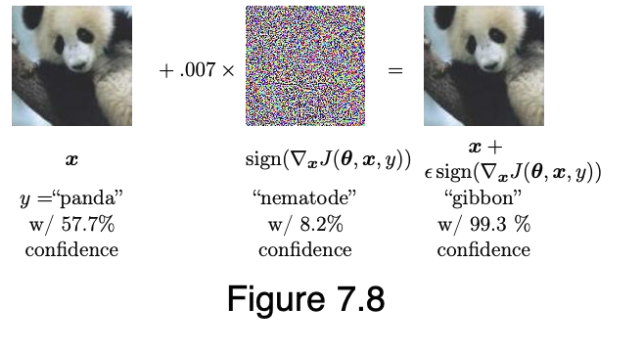
\includegraphics[scale=0.5]{assets/adversarial.png}

  You can see that adding some noise can wildly change the image. Using this in training can improve security. 
\end{center}
\subsubsection{Grokking}
Not yet peer reviewed, but is the phenomenon where training a long long time reduces the test error a lot
\begin{center}
  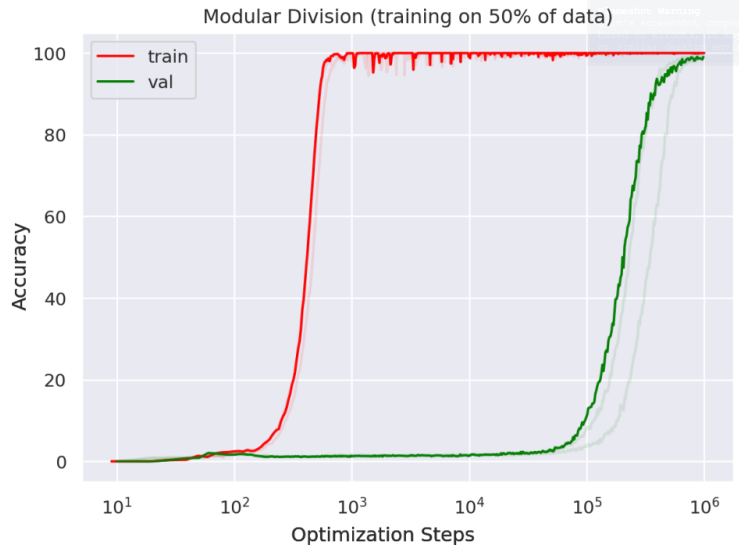
\includegraphics[scale=0.5]{assets/grokking.png}
\end{center}
But then there is also \textbf{anti-grokking} where if you run it even longer, it ends up overfitting. It's a new subject and not too explored.
\subsection{Regularization in DNNs: Dropout}
\begin{center}
  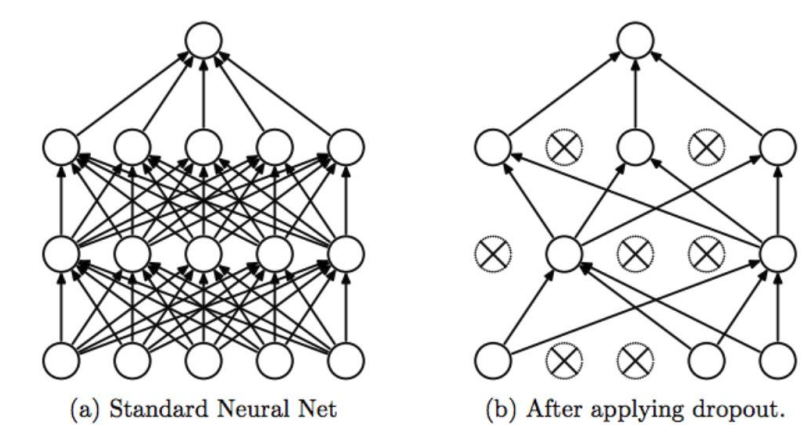
\includegraphics[scale=0.5]{assets/dropout.png}
\end{center}
Per learning cycle, we stochastically eliminate neurons with probability $p_{l}^{drop}$ in layer $l$. The intuition behind this is that we can't rely on any single feature, so we spread out the weights. It also avoids overfitting


He skipped a ton of slides here when doing the Lecture, I highly doubt it will come up in the exam.

\subsection{Convolutional Neural Networks}
So far we had many parameters, and fully connected feed-forward networks. This is not suitable for every task. For images, why should an object be treated differently based on location for example?

So the idea for CNN is local vs global processing of image features.

\begin{center}
  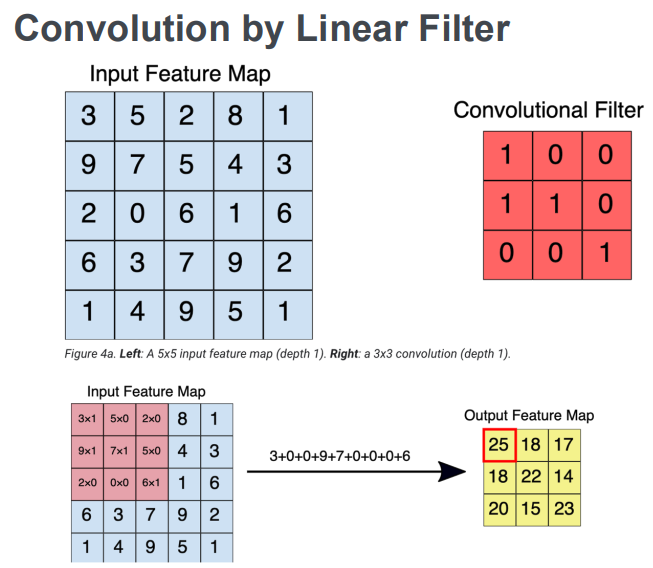
\includegraphics[scale=0.5]{assets/convolution_linear_filter.png}
\end{center}

\subsubsection{Reduce Dimensionality: Subsampling by pooling}
The main method is called \textbf{maxpool}. We have a pool of size $n\times n$ and we just get the max value. Same as a convolution, but we just access the max value. 

\begin{center}
  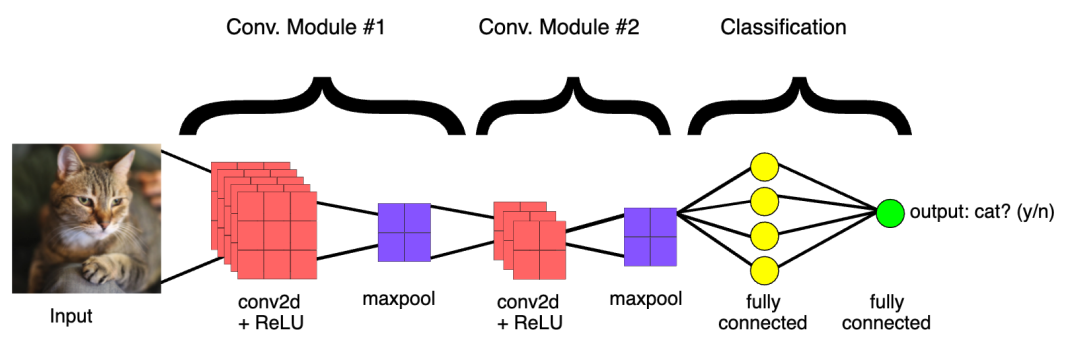
\includegraphics[scale=0.5]{assets/convolutional_neural_network.png}
\end{center}
\subsection{Recurrent Neural Networks}

\begin{center}
  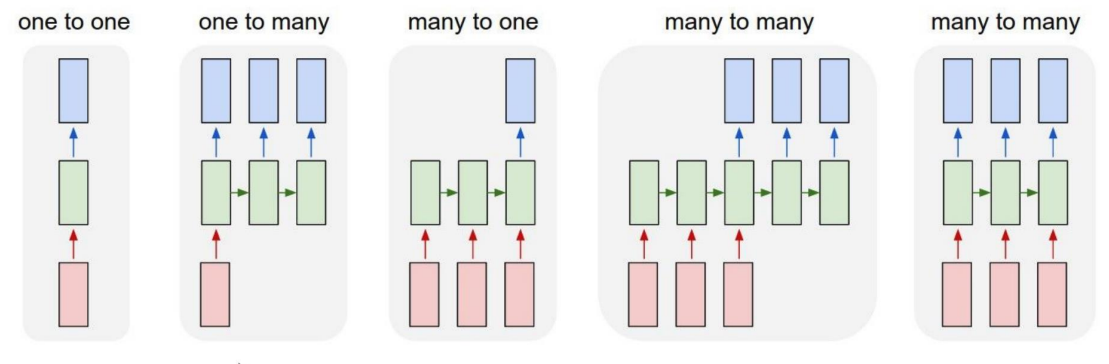
\includegraphics[scale=0.5]{assets/recurrent_nn.png}

  Our 'Vanilla' NN until now were the one to one model. The one-to-many could be image captioning (from image to sequence of words). The many-to-one could be Sentiment Classification (sequence of words to sentiment). Many-to-many could be machine translation (words to different words). And the last many-to-many could be video classification on frame level.
\end{center}

Recurrent Neural Networks are based on processing a vector $x$ by applying a \textbf{recurrence formula} at every time step
\[\underbrace{h_t}_{\text{new state}} = \underbrace{f_W}_{\text{function with params W}}(\underbrace{h_{t-1}}_{\text{old state}},\underbrace{x_t}_{\text{input vector at some time step}}) \] 

So the feedback from step $t$ to input at next time step $t+1$. Can be used for prediction of vehicle motion.
\subsection{When to use DNNs}
\subsubsection{Curse of Dimensionality}
\begin{itemize}
  \item Low Dimensionality: $x$ has few neighbors which are used to predict $y$
  \item High Dimensionality: $x$ has (too) many neighbors in roughly the same distance, hard to predict $y$
\end{itemize}
This is true for kNN, Decision Trees, SVMs, Bayes, etc.


Some last comments regarding manifolds, if they come up I will get angry $>:($


AND WE ARE DONE!!
\end{document}







